% document example:         https://www.overleaf.com/project/66dc4634e01fa87bf16cef97
% which is from tutorial:   https://www.overleaf.com/learn/latex/Beamer

\documentclass{beamer}
\usepackage[utf8]{inputenc}

\usepackage{nth} % to display nth in text

\usepackage{listings} % to have lstlisting environment

\usepackage{caption} % to remove prefix of caption, ex: "Figure:"

\usepackage{multirow}

\usepackage{romannum}

% https://tw.mirrors.cicku.me/ctan/macros/latex/contrib/minted/minted.pdf
% require to activate local python virtual environment with Pygments installed
% require "-shell-escape" option enabled when compiling TeX
\usepackage{minted} % for minted syntax highlighting environment
\usetheme{Madrid}
\usecolortheme{default} % default, beaver

\usepackage{tikz}
\usetikzlibrary{shapes.geometric, arrows}
\tikzstyle{block} = [rectangle,
rounded corners, 
minimum width=3cm, 
minimum height=1cm,
text centered,]
%draw=black, 
%fill=red!30]
\tikzstyle{path} = [rectangle,
rounded corners, 
minimum width=3cm, 
minimum height=1cm,
align=center,]
%text width=3cm,
\tikzstyle{miniblock} = [rectangle,
rounded corners, 
minimum width=3cm, 
minimum height=0.5cm,
text centered,]
\tikzstyle{minidecision} = [diamond,
minimum width=3cm,
minimum height=0.5cm,
text centered,]
\tikzstyle{arrow} = [thick,->,>=stealth]

%------------------------------------------------------------
%This block of code defines the information to appear in the
%Title page
\title[C project] %optional
{C project development and management on Linux}

\subtitle{A general introduction and \href{https://github.com/belongtothenight/autotools_init_setup}{\underline{project template}}}

\author[\href{https://github.com/belongtothenight/}{\underline{belongtothenight}}] % (optional)
{Da-Chuan Chen}

\date[20240907] % (optional)
{April \nth{7}, 2021}

%\logo{\includegraphics[height=1cm]{overleaf-logo}}

%End of title page configuration block
%------------------------------------------------------------



%------------------------------------------------------------
%The next block of commands puts the table of contents at the 
%beginning of each section and highlights the current section:

\AtBeginSection[]
{
  \begin{frame}
    \frametitle{Table of Contents}
    \tableofcontents[currentsection]
  \end{frame}
}
%------------------------------------------------------------

\begin{document}

%The next statement creates the title page.
\frame{\titlepage}

%---------------------------------------------------------
%This block of code is for the table of contents after
%the title page
\begin{frame}
\frametitle{Table of Contents}
\tableofcontents
\end{frame}
%---------------------------------------------------------

% - c example project
% - dev pipeline
%   1. c
%   2. compiler (can be expand into generating different stuff like man page)
%       - gcc (with example)
%       - g++
%       - clang
%       - llvm
%   3. various formats (for different purpose, static lib, dynamic lib, archive)
%   4. different install path for execution, linking...
% - build systems
%   - why?
%       - dependency checks and counter-measure (exist, version) (pkg-config)
%       - multiplatform support, portability (config.h, ./configure)
%       - automatically generate makefile
%       - version control (software-1.0.1)
%       - standardized build process
%       - standardized convensions (--prefix, --exec-prefix, /usr/bin, /usr/src, /usr/lib)
%       - incremental builds (only build files changed)
%       - library management (libtool)
%       - test after compilation
%   - make (automation tool)
%   - Autotools - make (a lot of GNU libraries) % https://docs.redhat.com/en/documentation/red_hat_enterprise_linux/6/html/developer_guide/cmd-autotools-upstreamdocs#cmd-autotools-upstreamdocs
%       - commands (./bootstrap.sh)
%   - CMake - make (a lot of C++ projects)
%       - commands
%   - Meson - ninja (a lot of GNOME)
%       - commands
%   - Yocto (out of bound)
%   - Buildroot (out of bound)
% - Autotools demo
%   - generate configure files
%   - prep for distribution
%       - multi-command
%       - single-command
%   - compile and installation
% - resolve issue when compiling from source
%   - distinguish build system and corresponding build commands
%   - dependency

\section{Example \textit{C} project}

\begin{frame}
    \frametitle{Example \textit{C} project}

    We are starting with an example \textit{C} project with \alert{multiple subdirectories} symbolizing a complex project structure. Each directory is responsible for a single binary. All besides the core functions should reside in the \texttt{lib} directory.

    \begin{figure}[H]
        \centering
        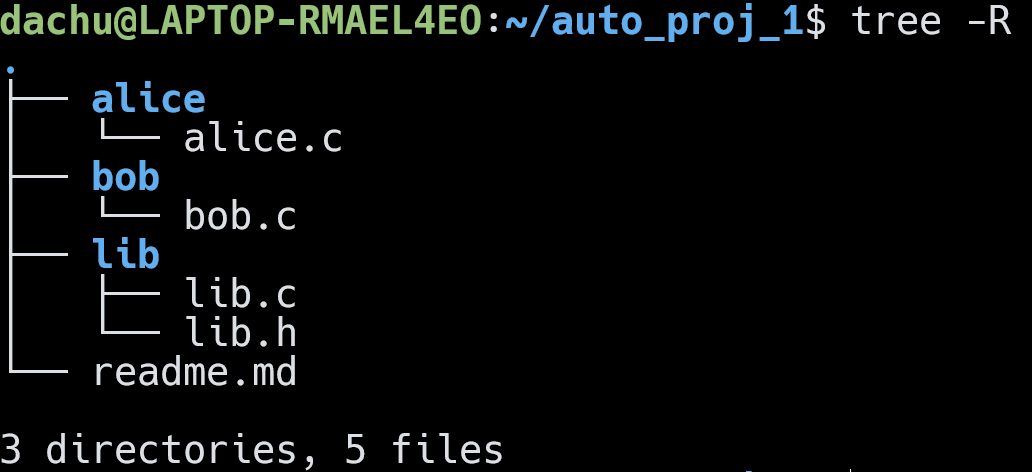
\includegraphics[width=0.8\textwidth]{../figure/init_state.png}
        \caption*{Tree structure of the example project.}
    \end{figure}
\end{frame}

\begin{frame}
    \frametitle{lib/lib.c \& lib/lib.h}

    \begin{figure}[hp]
        \centering
        \hfill
        \begin{minipage}{.8\textwidth}
            \inputminted[
                mathescape,
                linenos,
                autogobble,
                fontsize=\scriptsize,
            ]{bash}{E:\\GitHub\\presentation_in_LaTeX\\c_project_development\\proj\\auto_proj_init\\lib\\lib.c}
        \end{minipage}
        \hfill
        \caption*{Code of \texttt{lib/lib.c}.}
    \end{figure}

    \begin{figure}[H]
        \centering
        \hfill
        \begin{minipage}{.8\textwidth}
            \inputminted[
                mathescape,
                linenos,
                autogobble,
                fontsize=\scriptsize,
            ]{bash}{E:\\GitHub\\presentation_in_LaTeX\\c_project_development\\proj\\auto_proj_init\\lib\\lib.h}
        \end{minipage}
        \hfill
        \caption*{Code of \texttt{lib/lib.h}.}
    \end{figure}
\end{frame}

\begin{frame}
    \frametitle{alice/alice.c \& bob/bob.c}

    Both entry points \texttt{alice/alice.c} and \texttt{bob/bob.c} are dependent on the function \alert{\texttt{print\_hello}}.

    \begin{figure}[hp]
        \centering
        \hfill
        \begin{minipage}{.4\textwidth}
            \inputminted[
                mathescape,
                linenos,
                autogobble,
                fontsize=\scriptsize,
            ]{c}{E:\\GitHub\\presentation_in_LaTeX\\c_project_development\\proj\\auto_proj_init\\alice\\alice.c}
            \caption*{Code of \texttt{alice/alice.c}.}
        \end{minipage}%
        \hfill
        \begin{minipage}{.4\textwidth}
            \centering
            \inputminted[
                mathescape,
                linenos,
                autogobble,
                fontsize=\scriptsize,
            ]{c}{E:\\GitHub\\presentation_in_LaTeX\\c_project_development\\proj\\auto_proj_init\\bob\\bob.c}
            \caption*{Code of \texttt{bob/bob.c}.}
        \end{minipage}
        \hfill
    \end{figure}

\end{frame}

\section{Development process}

\begin{frame}
    \frametitle{Development process}

    \begin{enumerate}
        \item \footnotesize Select building target.
            \begin{itemize}
                \item \scriptsize Binary
                \item \scriptsize Library: static (\texttt{*.o}) and shared (\texttt{*.so})
                \item \scriptsize Archive of library (\texttt{*.a})
                \item \scriptsize Libtool library (\texttt{*.la})
            \end{itemize}
        \item \footnotesize Project positioning.
            \begin{itemize}
                \item \scriptsize Multi-platform support (like CPU architectures, available resouorces)
                \item \scriptsize Embedded platform
                \item \scriptsize Library dependency and availability
                \item \scriptsize Distribution method (like APT, SourceForge, GitHub, binary, source code)
            \end{itemize}
        \item \footnotesize Code in \textit{C}.
        \item \footnotesize Build with compiler. (compile, link, $\cdots$)
            \begin{itemize}
                \item \scriptsize Language standards (like \textit{C99})
                \item \scriptsize Flags (like \texttt{-Wall})
                \item \scriptsize Dependent library headers
                \item \scriptsize Dependent library pre-compiled binary
                \item \scriptsize Code optimization (like \texttt{-O2 -O3})
                \item \scriptsize Debugging information
                \item \scriptsize Debug and profiling (like Valgrind, sanitizers, FlameGraph)
                    \begin{itemize}
                        \item \tiny Memory (heap) error (memory leak)
                        \item \tiny Thread error (racing)
                        \item \tiny Cache
                        \item \tiny Branch-prediction
                    \end{itemize}
            \end{itemize}
        \item \footnotesize Install, uninstall, system integration.
    \end{enumerate}
\end{frame}

\begin{frame}
    \frametitle{Deployment checks}

    How can we ensure that once the project is built, it can be executed correctly, consistently, and without problems?

    \begin{itemize}
        \item Pre-Build check list
            \begin{itemize}
                \item Compiler: \texttt{gcc}, \texttt{g++}, \texttt{clang}, \texttt{llvm}, $\cdots$
                \item Required software, library, function
                \item Version (like $>1.0.0$)
                \item Command execution location in project
            \end{itemize}
        \item Post-Build
            \begin{itemize}
                \item Can be executed or linked both locally and at the installing location
                \item Execution result is correct and consistent
            \end{itemize}
    \end{itemize}

    The thing is, coding \textit{C} is just a fraction of creating binaries and libraries.
\end{frame}

\begin{frame}
    \frametitle{Manual compile}
    
    % https://tex.stackexchange.com/questions/5818/how-to-center-a-listing

    If the project is not complicated, manually compiling everything or using a Bash script is acceptable. However, installing, uninstalling, and cleaning are not implemented.

    \begin{figure}[hp]
        \centering
        \hfill
        \begin{minipage}{.9\textwidth}
            \inputminted[
                mathescape,
                linenos,
                autogobble,
                fontsize=\scriptsize,
                firstline=2,
                lastline=4,
            ]{bash}{E:\\GitHub\\presentation_in_LaTeX\\c_project_development\\script\\term_cmd.sh}
        \end{minipage}
        \hfill
        \caption*{Commands for manual \texttt{gcc} compilation.}
    \end{figure}

    \begin{figure}[H]
        \centering
        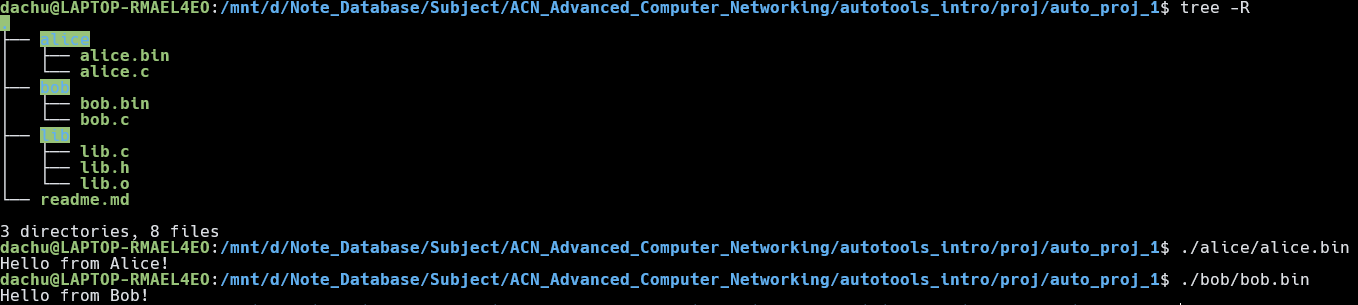
\includegraphics[width=0.9\textwidth]{../figure/manual_compile.png}
        \caption*{Tree structure and execution results after compilation.}
    \end{figure}
\end{frame}

\section{Build systems}

\begin{frame}
    \frametitle{Makefile}

    \begin{figure}[H]
        \centering
        \hfill
        \begin{minipage}{.95\textwidth}
            \inputminted[
                mathescape,
                linenos,
                autogobble,
                fontsize=\tiny,
            ]{makefile}{E:\\GitHub\\presentation_in_LaTeX\\c_project_development\\script\\Makefile}
        \end{minipage}
        \hfill
        \caption*{Example of a Makefile with build and clean targets.}
    \end{figure}
\end{frame}

\begin{frame}
    \frametitle{Makefile compile}

    \begin{figure}[H]
        \centering
        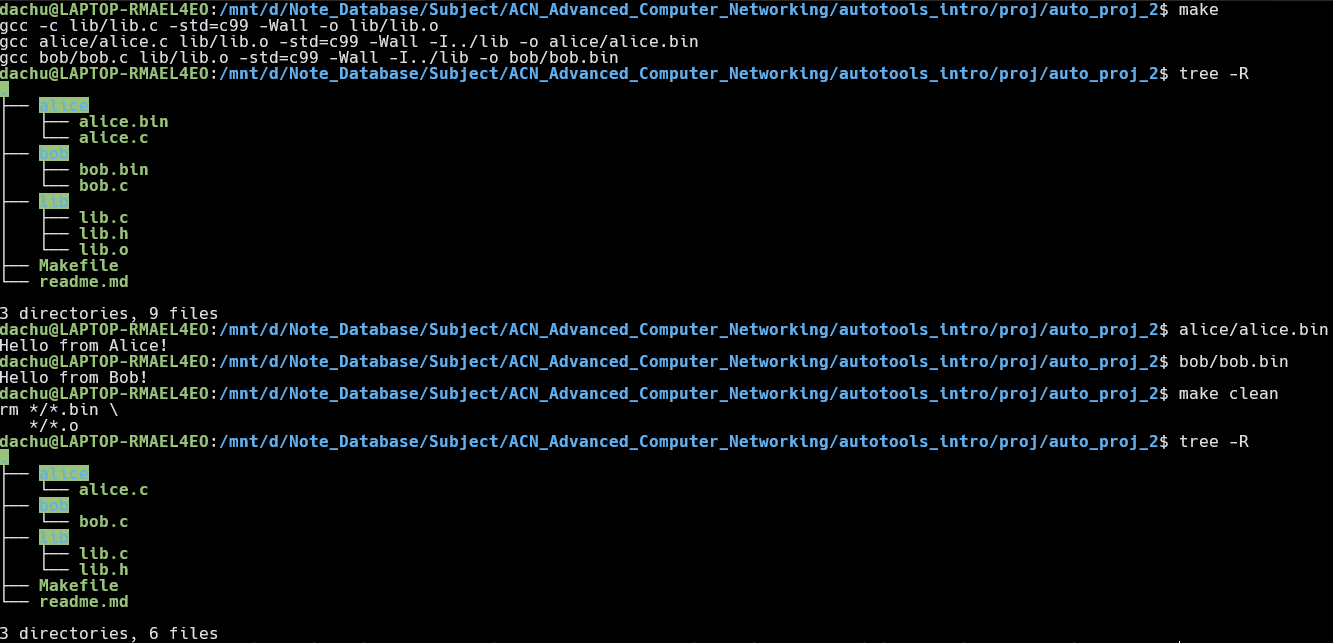
\includegraphics[width=0.9\textwidth]{../figure/makefile_compile.png}
        \caption*{Tree structure and execution results after compilation.}
    \end{figure}
\end{frame}

\begin{frame}
    \frametitle{Makefile}

    \begin{itemize}
        \item Work similar to \textit{Bash}
        \item Can specify a single target with all of its dependency compiled
        \item Takes a lot of time to configure if there are too many files
        \item All actions include \alert{building}, \alert{installing}, \alert{uninstalling}, and \alert{clearing} require knowledge of convension and manual configuration
    \end{itemize}
\end{frame}

\begin{frame}
    \frametitle{Development pipeline with build systems}

    \begin{center}
        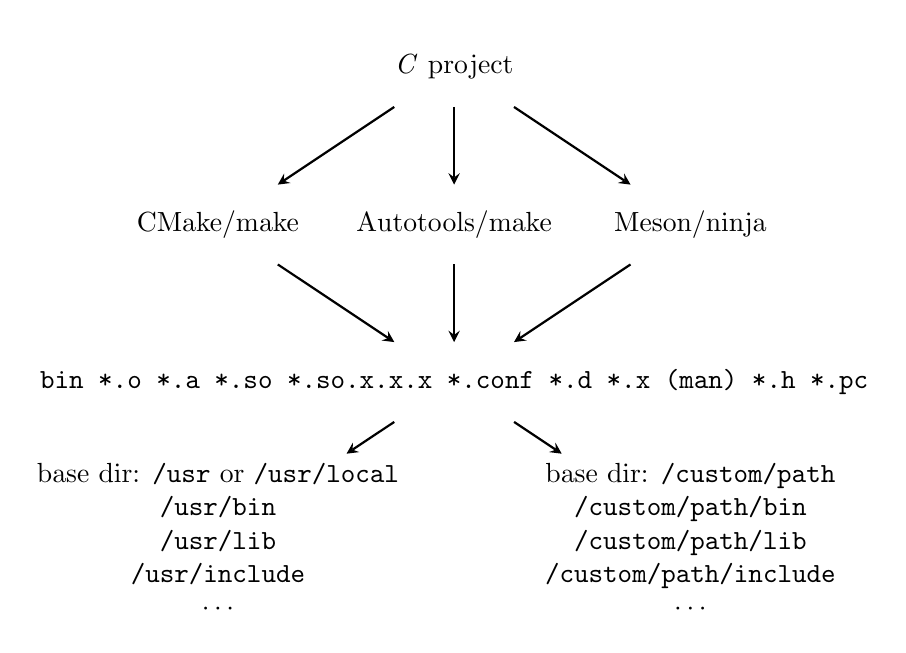
\begin{tikzpicture}[node distance=2cm]
            \node (start) [block] {\textit{C} project};
            \node (bs1) [block, below of=start] {Autotools/make};
            \node (bs2) [block, left of=bs1, xshift=-1cm] {CMake/make};
            \node (bs3) [block, right of=bs1, xshift=1cm] {Meson/ninja};
            \node (f) [block, below of=bs1] {\texttt{bin *.o *.a *.so *.so.x.x.x *.conf *.d *.x (man) *.h *.pc}};
            \node (def) [path, below of=f, xshift=-3cm] {base dir: \texttt{/usr} or \texttt{/usr/local}\\
                \texttt{/usr/bin}\\
                \texttt{/usr/lib}\\
                \texttt{/usr/include}\\
                $\cdots$};
            \node (gen) [path, below of=f, xshift=3cm] {base dir: \texttt{/custom/path}\\
                \texttt{/custom/path/bin}\\
                \texttt{/custom/path/lib}\\
                \texttt{/custom/path/include}\\
                $\cdots$};

            \draw [arrow] (start) -- (bs1);
            \draw [arrow] (start) -- (bs2);
            \draw [arrow] (start) -- (bs3);
            \draw [arrow] (bs1) -- (f);
            \draw [arrow] (bs2) -- (f);
            \draw [arrow] (bs3) -- (f);
            \draw [arrow] (f) -- (def);
            \draw [arrow] (f) -- (gen);
        \end{tikzpicture}
    \end{center}
\end{frame}

\begin{frame}
    \frametitle{Why build systems}

    \begin{itemize}
        \item Dependency checks on existence and version (pkg-config)
        \item Multi-platform portability (\texttt{config.h} and \texttt{./configure})
        \item Standardized build process
        \item Standardized convensions (like \texttt{./configure --prefix=/path --exec-path=/path})
        \item Incremental build, which only build changed files
        \item Library management (\texttt{libtool})
        \item Run tests after compilation if existed
    \end{itemize}
\end{frame}

\begin{frame}
    \frametitle{Common build systems}

    \begin{center}
        \footnotesize
        \begin{tabular}{ c | c c c }
            \hline
            Build system & Autotools/make & CMake/make & Meson/ninja \\
            \hline
            Common usecase & GNU libraries & \textit{C++} projects & GNOME \\
            \hline
            Common files & \texttt{configure.ac} & \texttt{CMakeLists.txt} & \texttt{meson.build} \\
            to identify & \texttt{Makefile.am} & & \texttt{meson.options} \\
            \hline
            \multirow[t]{6}{*}{Build command} & \scriptsize\texttt{cd \$project\_dir} & \scriptsize\texttt{cd \$project\_dir} & \scriptsize\texttt{cd \$project\_dir} \\
            & \scriptsize\texttt{./configure} & \scriptsize\texttt{mkdir build} & \scriptsize\texttt{meson setup \_build} \\
            & \scriptsize\texttt{make} & \scriptsize\texttt{cd build} & \scriptsize\texttt{meson compile -C \_build} \\
            & \scriptsize\texttt{make install} & \scriptsize\texttt{cmake ..} & \scriptsize\texttt{meson install -C \_build} \\
            & & \scriptsize\texttt{make} & \\
            & & \scriptsize\texttt{make install} & \\
            \hline
        \end{tabular}
    \end{center}
\end{frame}

\section{Autotools demo}

%https://www.gnu.org/savannah-checkouts/gnu/automake/manual/automake.html

\begin{frame}
    \frametitle{Steps for creating a \textit{C} project managed by Autotools}

    \alert{Phase \Romannum{1}: Initial setup}

    \begin{enumerate}
        \item Create and configure main \texttt{Makefile.am}.
        \item Create and configure \texttt{Makefile.am} in every subdirectories.
        \item Use \texttt{autoscan} to generate the starting point of \texttt{configure.scan}.
        \item Modify \texttt{configure.scan} with project settings into \texttt{configure.ac}.
        \item Use \texttt{autoreconf} to generate \texttt{./configure}.
    \end{enumerate}
    
\end{frame}

\begin{frame}
    \frametitle{Steps for creating a \textit{C} project managed by Autotools}

    \alert{Phase \Romannum{2}: Build}

    \begin{enumerate}
        \item Execute \texttt{./configure} to generate Makefiles.
        \item Execute \texttt{make} in the root directory of the project to build. (include testing)
        \item Execute \texttt{make install} in the root directory of the project to install.
    \end{enumerate}

    \alert{Phase \Romannum{3}: Prepare for distribution}

    \begin{enumerate}
        \item Execute \texttt{make clean} to remove build results in project.
        \item Execute \texttt{make distclean} to remove everything generated with \texttt{./configure}.
        \item Compress the directory (\texttt{*.tar.gz}) for release.
    \end{enumerate}
\end{frame}

\subsection{Phase \Romannum{1}: Initial setup}

\begin{frame}
    \frametitle{\Romannum{1}: ./Makefile.am}

    \begin{figure}[H]
        \centering
        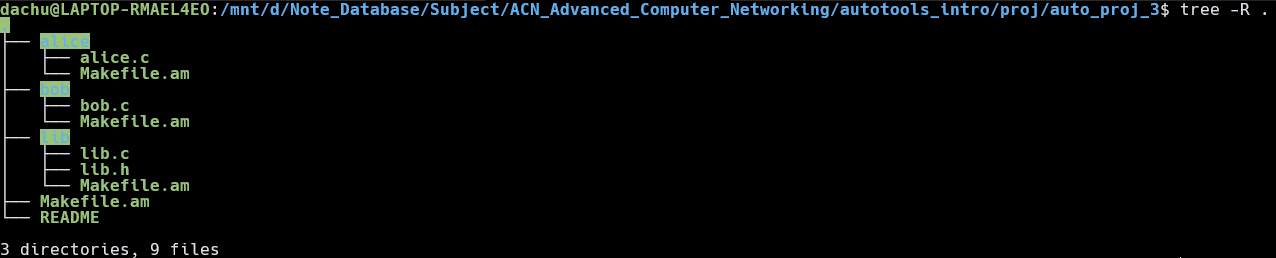
\includegraphics[width=0.9\textwidth]{../figure/autotool_init.png}
        \caption*{Tree structure after creating \texttt{Makefile.am}.}
    \end{figure}

    \begin{figure}[hp]
        \centering
        \hfill
        \begin{minipage}{.9\textwidth}
            \inputminted[
                mathescape,
                linenos,
                autogobble,
                fontsize=\scriptsize,
            ]{makefile}{E:\\GitHub\\presentation_in_LaTeX\\c_project_development\\script\\Makefile_root.am}
        \end{minipage}
        \hfill
        \caption*{Code for \texttt{./Makefile.am}.}
    \end{figure}
\end{frame}

\begin{frame}
    \frametitle{\Romannum{1}: Makefile.am for directory \texttt{alice} to build a binary}

    \begin{figure}[hp]
        \centering
        \hfill
        \begin{minipage}{.9\textwidth}
            \inputminted[
                mathescape,
                linenos,
                autogobble,
                fontsize=\tiny,
            ]{makefile}{E:\\GitHub\\presentation_in_LaTeX\\c_project_development\\script\\Makefile_alice.am}
        \end{minipage}
        \hfill
        \caption*{Code for \texttt{./alice/Makefile.am}.}
    \end{figure}
\end{frame}

\begin{frame}
    \frametitle{\Romannum{1}: Makefile.am for directories \texttt{bob} to build a binary}

    \begin{figure}[hp]
        \centering
        \hfill
        \begin{minipage}{.9\textwidth}
            \inputminted[
                mathescape,
                linenos,
                autogobble,
                fontsize=\tiny,
            ]{makefile}{E:\\GitHub\\presentation_in_LaTeX\\c_project_development\\script\\Makefile_bob.am}
        \end{minipage}
        \hfill
        \caption*{Code for \texttt{./bob/Makefile.am}.}
    \end{figure}
\end{frame}

\begin{frame}
    \frametitle{\Romannum{1}: Makefile.am for directory \texttt{lib} to build a LibTool library}

    \begin{figure}[hp]
        \centering
        \hfill
        \begin{minipage}{.9\textwidth}
            \inputminted[
                mathescape,
                linenos,
                autogobble,
                fontsize=\tiny,
            ]{makefile}{E:\\GitHub\\presentation_in_LaTeX\\c_project_development\\script\\Makefile_lib.am}
        \end{minipage}
        \hfill
        \caption*{Code for \texttt{./lib/Makefile.am}.}
    \end{figure}
\end{frame}

\begin{frame}
    \frametitle{\Romannum{1}: \texttt{autoscan} for configure template \texttt{configure.scan}}

    \begin{figure}[hp]
        \centering
        \hfill
        \begin{minipage}{.9\textwidth}
            \inputminted[
                mathescape,
                linenos,
                autogobble,
                fontsize=\tiny,
            ]{bash}{E:\\GitHub\\presentation_in_LaTeX\\c_project_development\\script\\configure.scan}
        \end{minipage}
        \hfill
        \caption*{Scan result of the project structure in \texttt{configure.scan}.}
    \end{figure}
\end{frame}

\begin{frame}
    \frametitle{\Romannum{1}: \texttt{autoscan} for configure template \texttt{configure.ac}}

    \begin{figure}[hp]
        \centering
        \hfill
        \begin{minipage}{.9\textwidth}
            \inputminted[
                mathescape,
                linenos,
                autogobble,
                fontsize=\tiny,
                firstline=1,
                lastline=23,
            ]{bash}{E:\\GitHub\\presentation_in_LaTeX\\c_project_development\\script\\configure.ac}
        \end{minipage}
        \hfill
        \caption*{Modified \texttt{configure.ac}. (part 1)}
    \end{figure}
\end{frame}

\begin{frame}
    \frametitle{\Romannum{1}: \texttt{autoscan} for configure template \texttt{configure.ac}}

    \begin{figure}[hp]
        \centering
        \hfill
        \begin{minipage}{.9\textwidth}
            \inputminted[
                mathescape,
                linenos,
                autogobble,
                fontsize=\tiny,
                firstline=25,
                lastline=53,
            ]{bash}{E:\\GitHub\\presentation_in_LaTeX\\c_project_development\\script\\configure.ac}
        \end{minipage}
        \hfill
        \caption*{Modified \texttt{configure.ac}. (part 2)}
    \end{figure}
\end{frame}

\begin{frame}
    \frametitle{\Romannum{1}: \texttt{autoreconf -iv}}

    \begin{figure}[H]
        \centering
        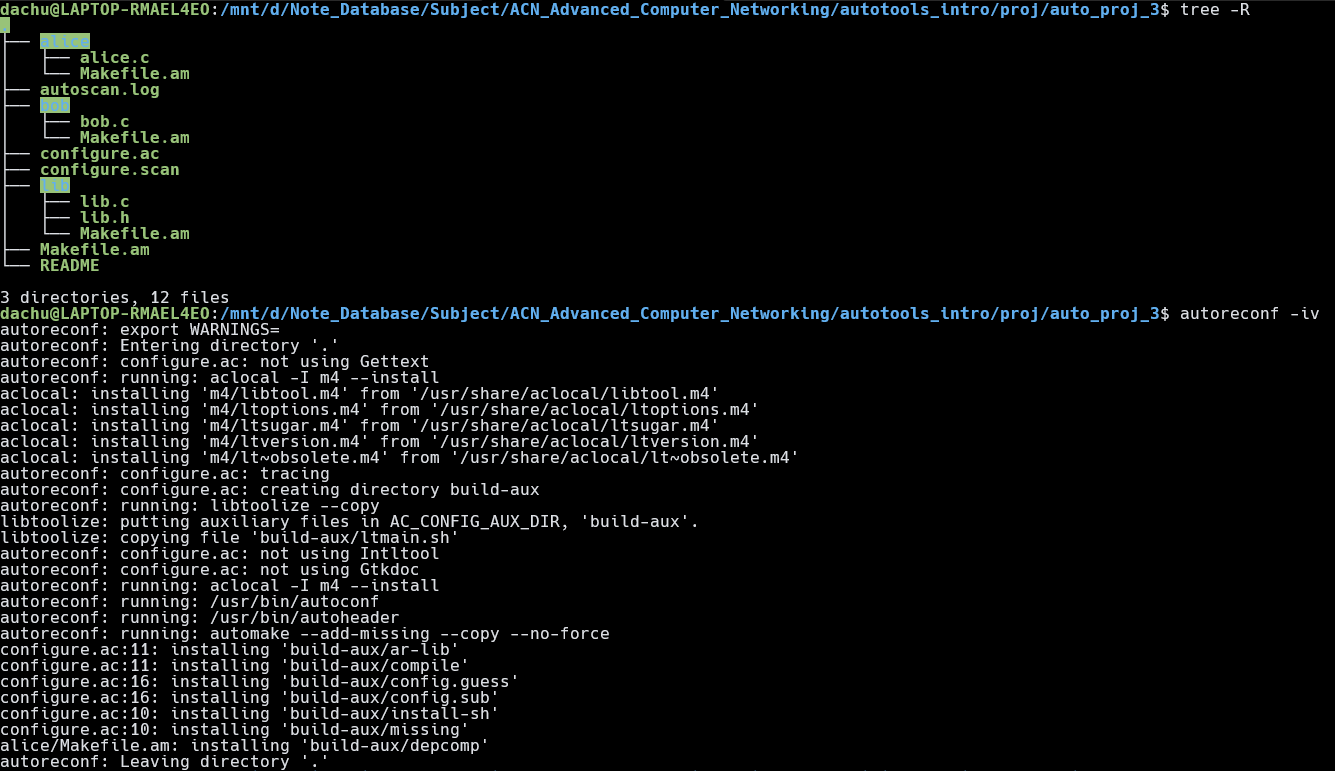
\includegraphics[width=0.9\textwidth]{../figure/autotool_1.png}
        \caption*{Generate auxiliary files.}
    \end{figure}
\end{frame}

\begin{frame}
    \frametitle{\Romannum{1}: \texttt{autoreconf -iv}}

    \begin{figure}[H]
        \centering
        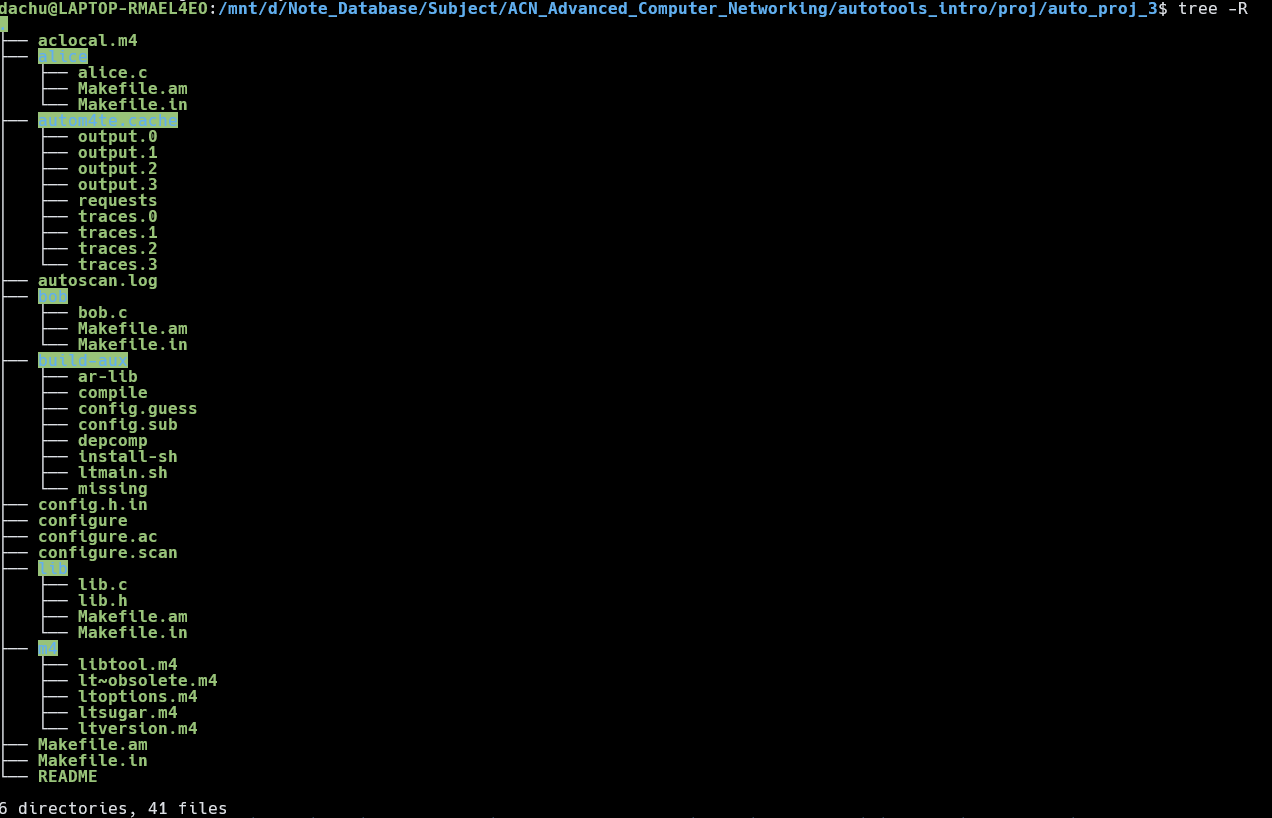
\includegraphics[width=0.9\textwidth]{../figure/autotool_2.png}
        \caption*{Tree structure of generate auxiliary files.}
    \end{figure}
\end{frame}

\subsection{Phase \Romannum{2}: Build}

\begin{frame}
    \frametitle{\Romannum{2}: \texttt{./configure}}

    \begin{figure}[H]
        \centering
        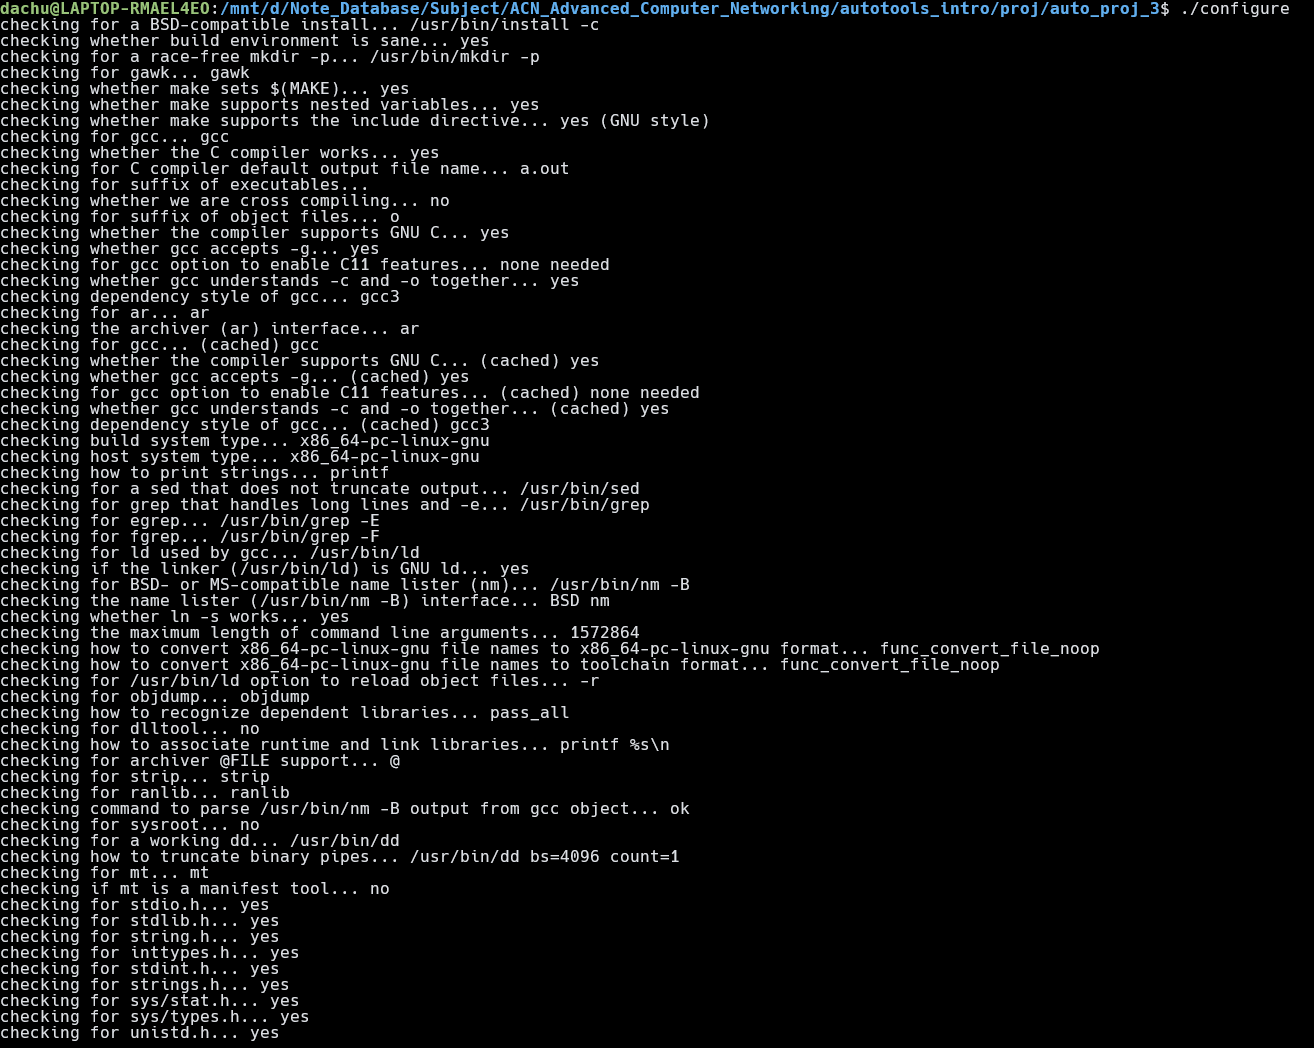
\includegraphics[width=0.7\textwidth]{../figure/autotool_3.png}
        \caption*{Generate Makefile for installing platform. (part 1)}
    \end{figure}
\end{frame}

\begin{frame}
    \frametitle{\Romannum{2}: \texttt{./configure}}

    \begin{figure}[H]
        \centering
        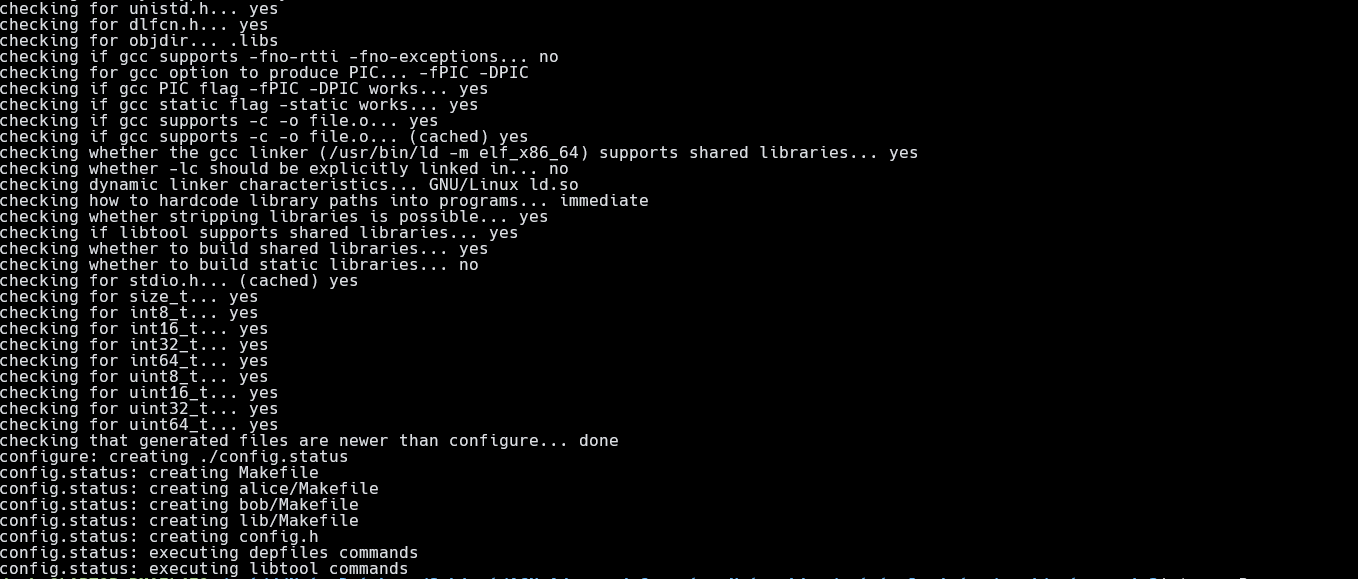
\includegraphics[width=0.8\textwidth]{../figure/autotool_4.png}
        \caption*{Generate Makefile for installing platform. (part 2)}
    \end{figure}
\end{frame}

\begin{frame}
    \frametitle{\Romannum{2}: \texttt{./configure}}

    \begin{figure}[H]
        \centering
        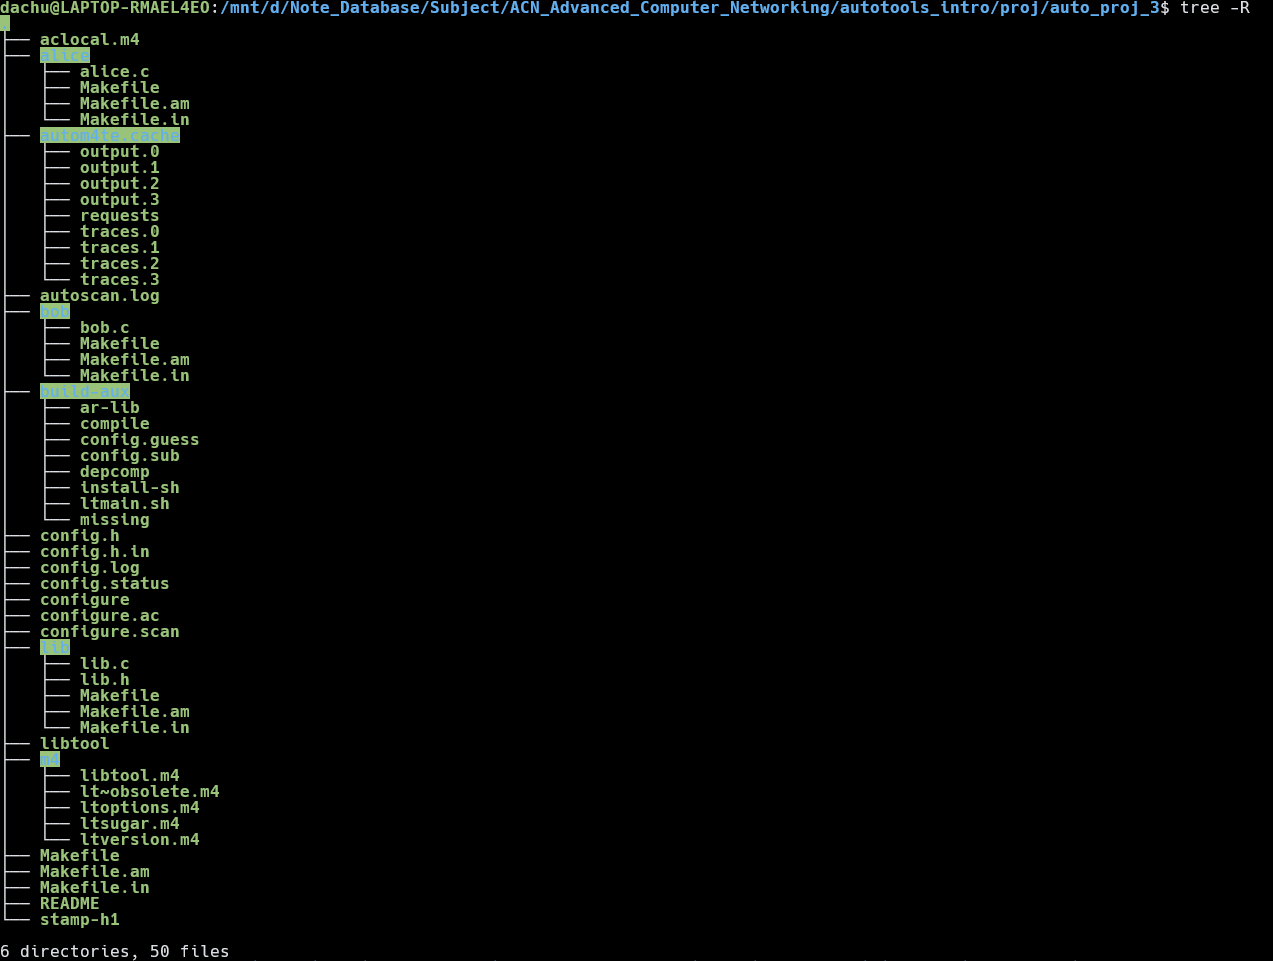
\includegraphics[width=0.7\textwidth]{../figure/autotool_5.png}
        \caption*{Tree structure of generated files including \texttt{Makefile}.}
    \end{figure}
\end{frame}

\begin{frame}
    \frametitle{\Romannum{2}: \texttt{make}}

    \begin{figure}[H]
        \centering
        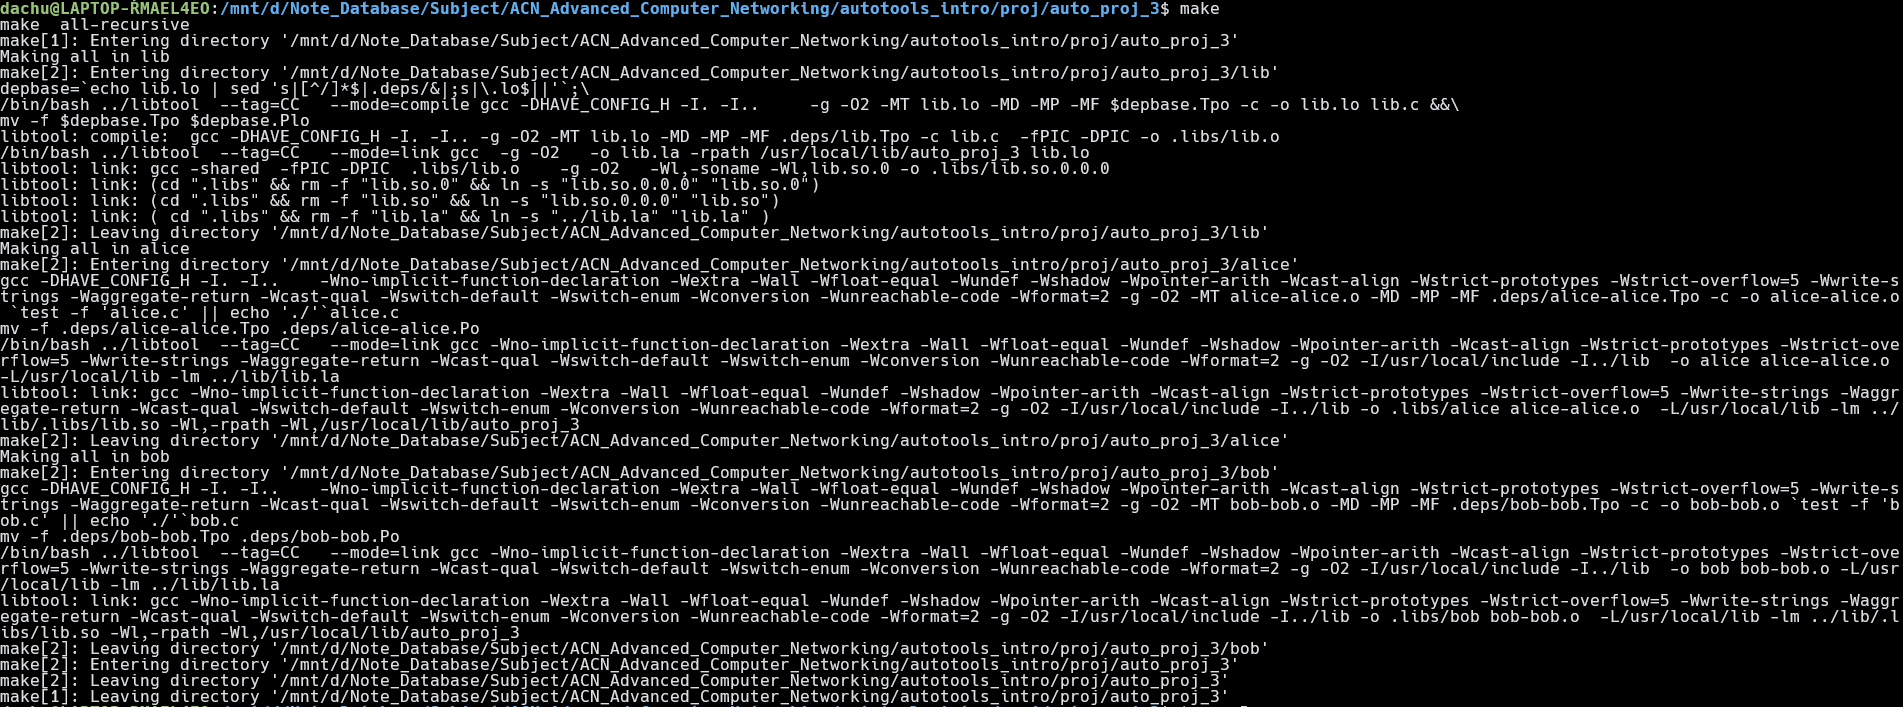
\includegraphics[width=0.95\textwidth]{../figure/autotool_6.png}
        \caption*{Project building.}
    \end{figure}
\end{frame}

\begin{frame}
    \frametitle{\Romannum{2}: \texttt{make}}

    \begin{figure}[H]
        \centering
        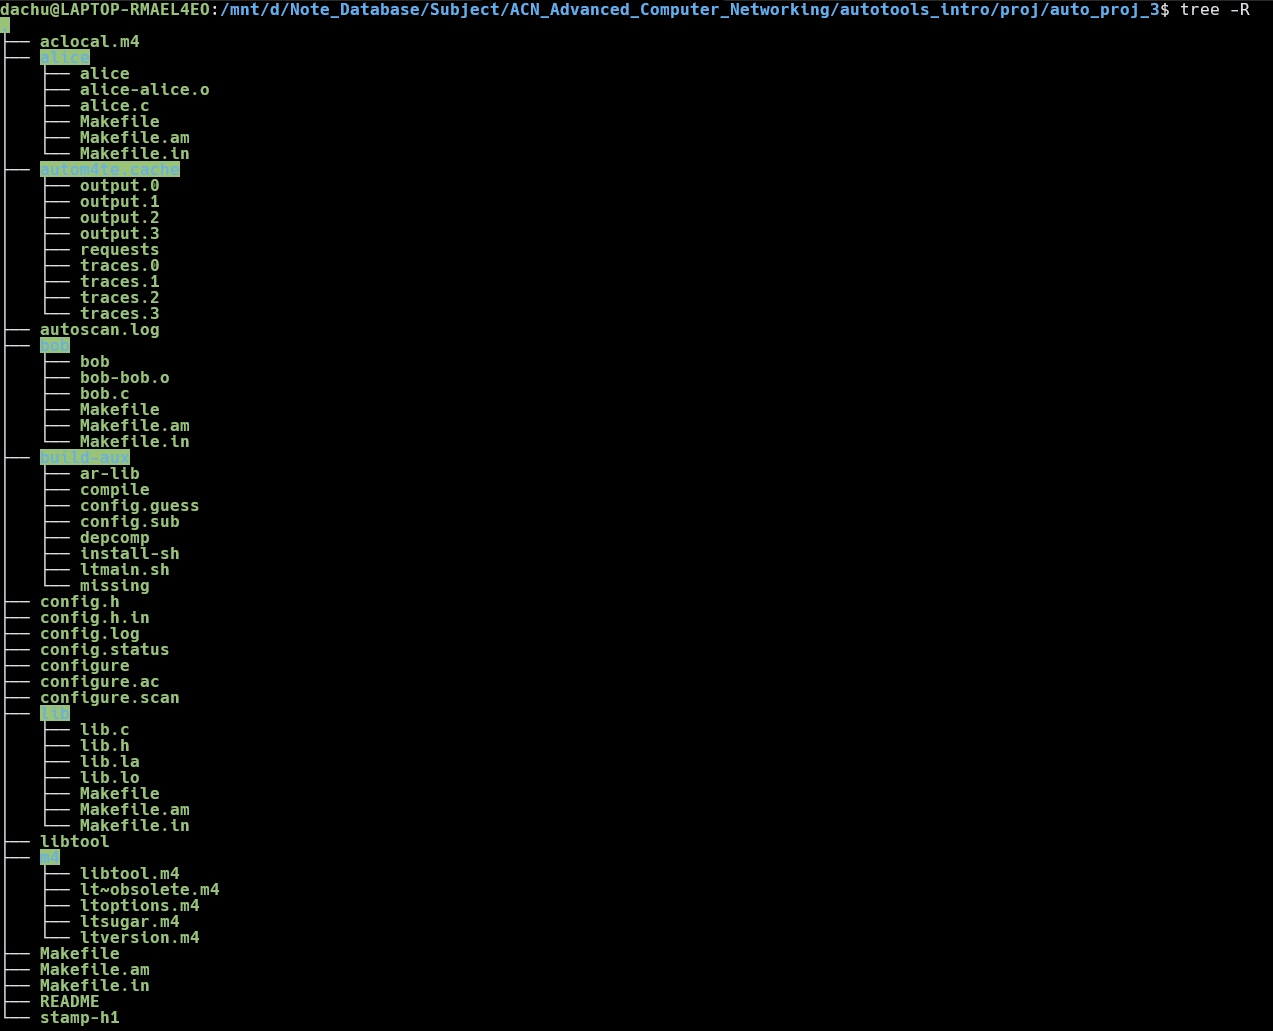
\includegraphics[width=0.7\textwidth]{../figure/autotool_7.png}
        \caption*{Tree structure of built project.}
    \end{figure}
\end{frame}

\begin{frame}
    \frametitle{\Romannum{2}: \texttt{make install}}

    \begin{figure}[H]
        \centering
        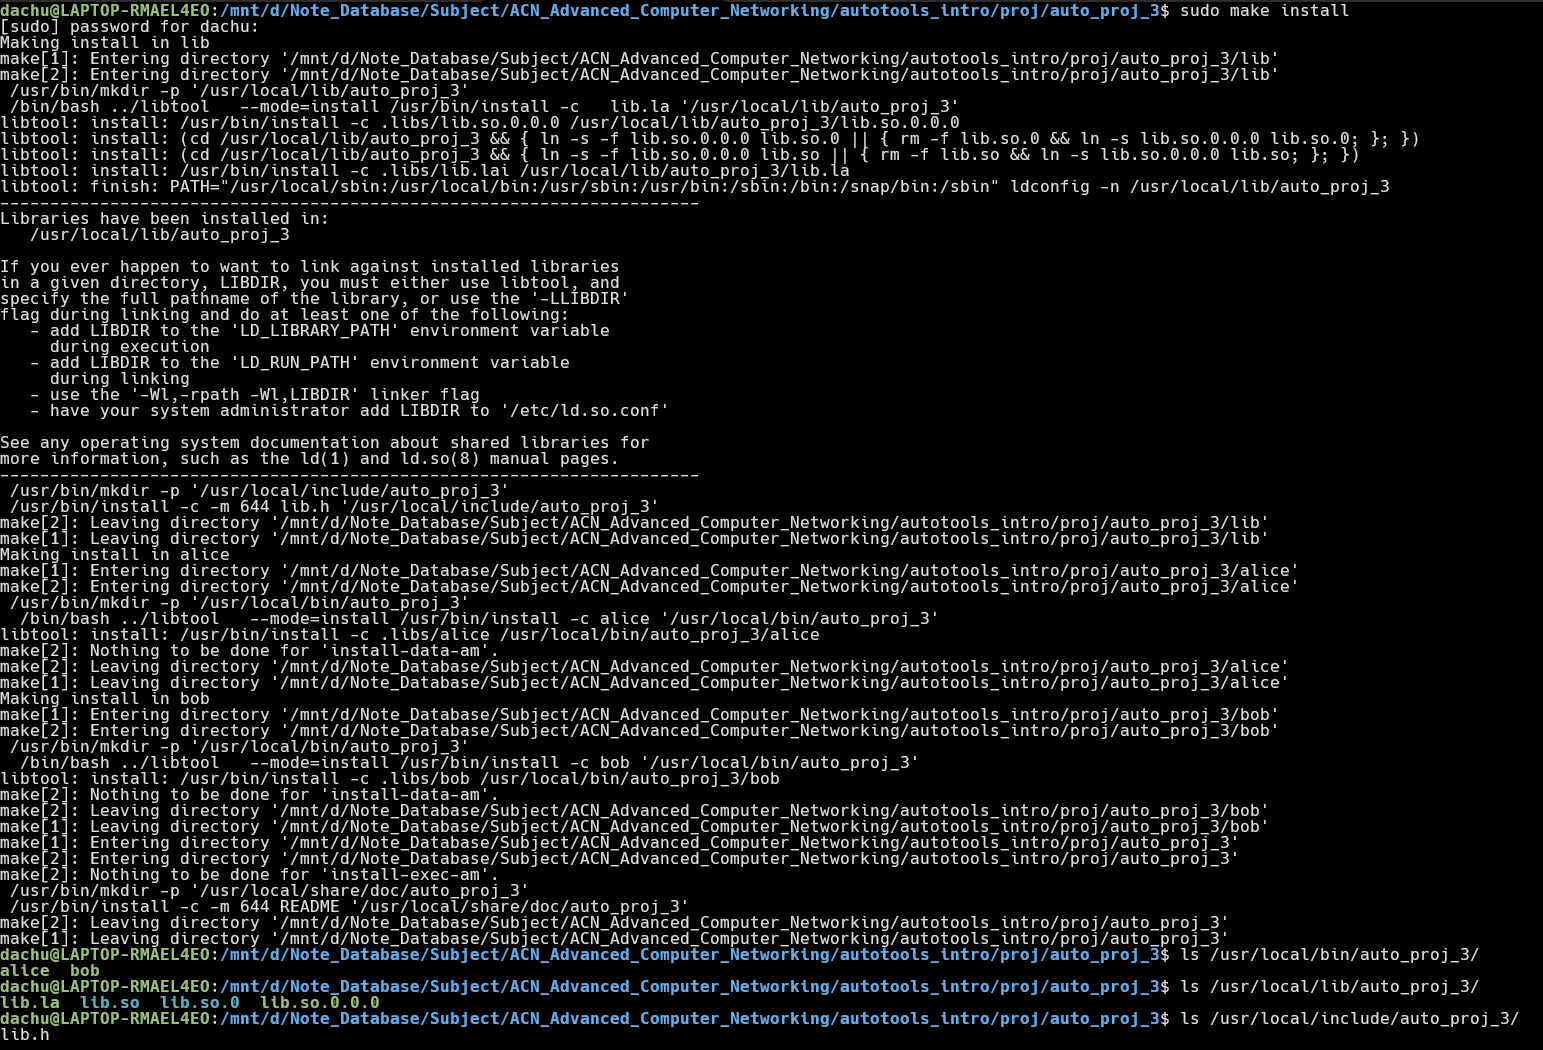
\includegraphics[width=0.8\textwidth]{../figure/autotool_8.png}
        \caption*{Execution result and installed files.}
    \end{figure}
\end{frame}

\begin{frame}
    \frametitle{\Romannum{2}: \texttt{make uninstall}}

    \begin{figure}[H]
        \centering
        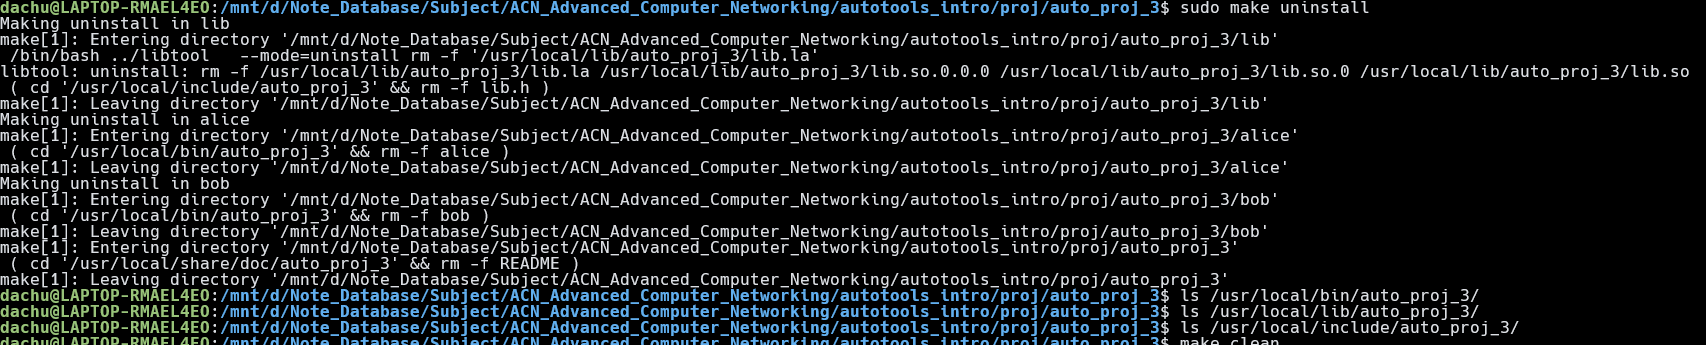
\includegraphics[width=0.9\textwidth]{../figure/autotool_9.png}
        \caption*{Removing all installed files.}
    \end{figure}
\end{frame}

\subsection{Phase \Romannum{3}: Prepare for distribution}

\begin{frame}
    \frametitle{\Romannum{3}: \texttt{make clean}}

    \begin{figure}[H]
        \centering
        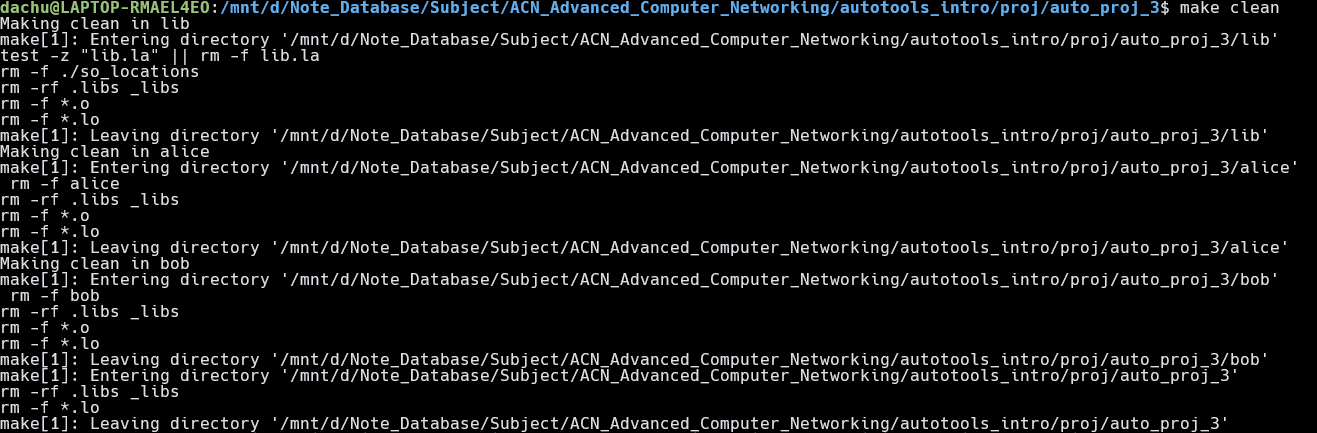
\includegraphics[width=0.9\textwidth]{../figure/autotool_10.png}
        \caption*{Remove all compiled files.}
    \end{figure}
\end{frame}

\begin{frame}
    \frametitle{\Romannum{3}: \texttt{make clean}}

    \begin{figure}[H]
        \centering
        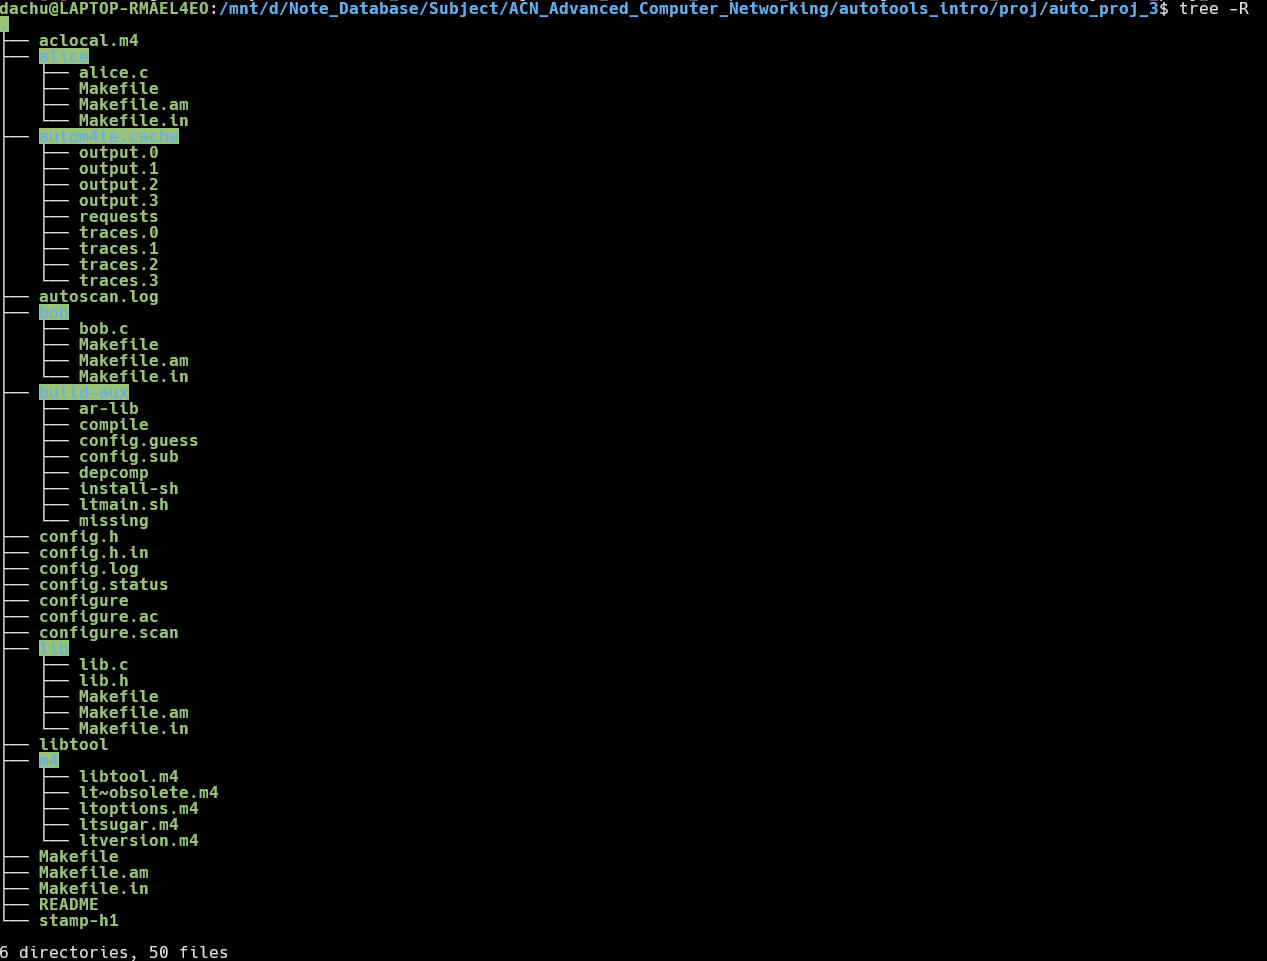
\includegraphics[width=0.7\textwidth]{../figure/autotool_11.png}
        \caption*{Tree structure after execution.}
    \end{figure}
\end{frame}

\begin{frame}
    \frametitle{\Romannum{3}: \texttt{make distclean}}

    \begin{figure}[H]
        \centering
        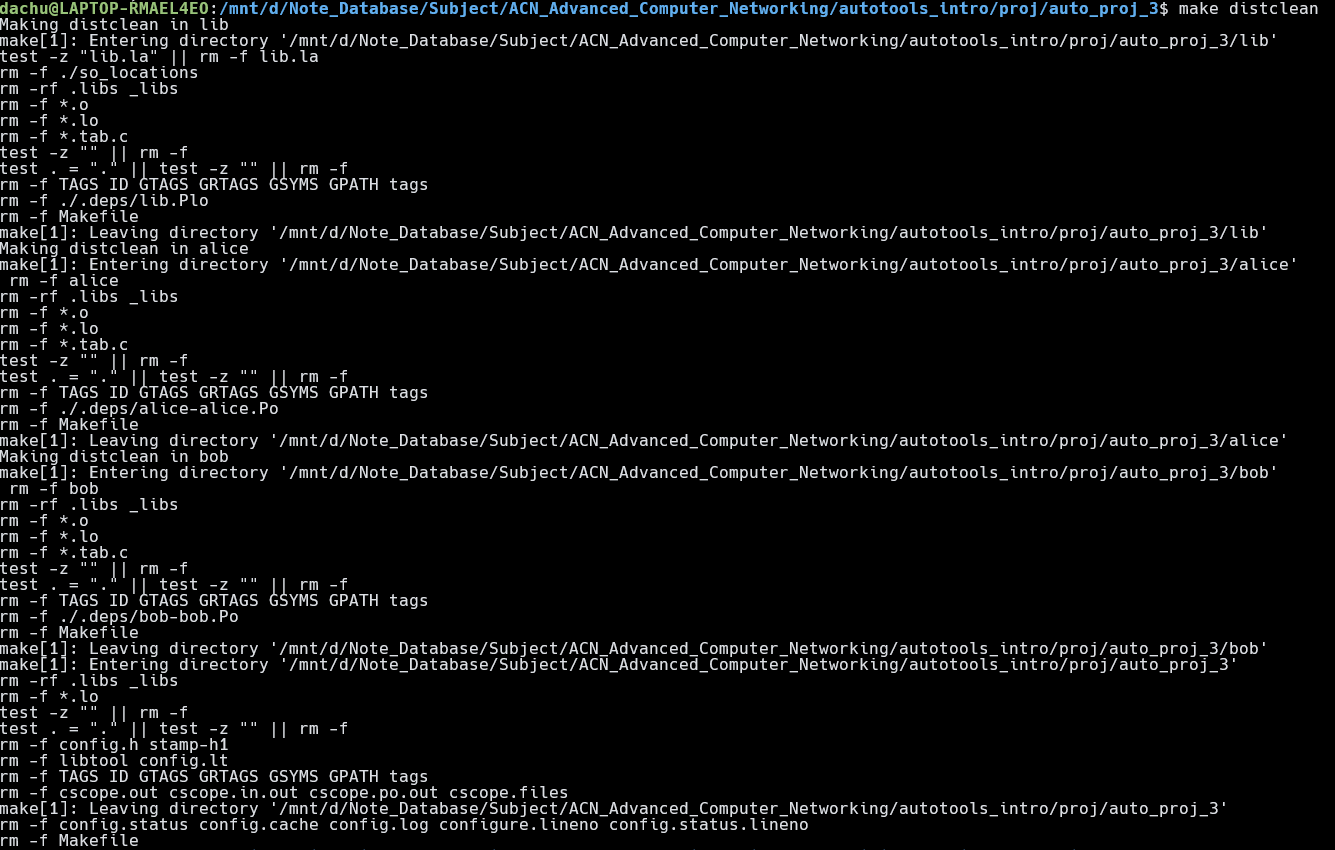
\includegraphics[width=0.8\textwidth]{../figure/autotool_12.png}
        \caption*{Remove almost all files generated from \texttt{./configure}.}
    \end{figure}
\end{frame}

\begin{frame}
    \frametitle{\Romannum{3}: \texttt{make distclean}}

    \begin{figure}[H]
        \centering
        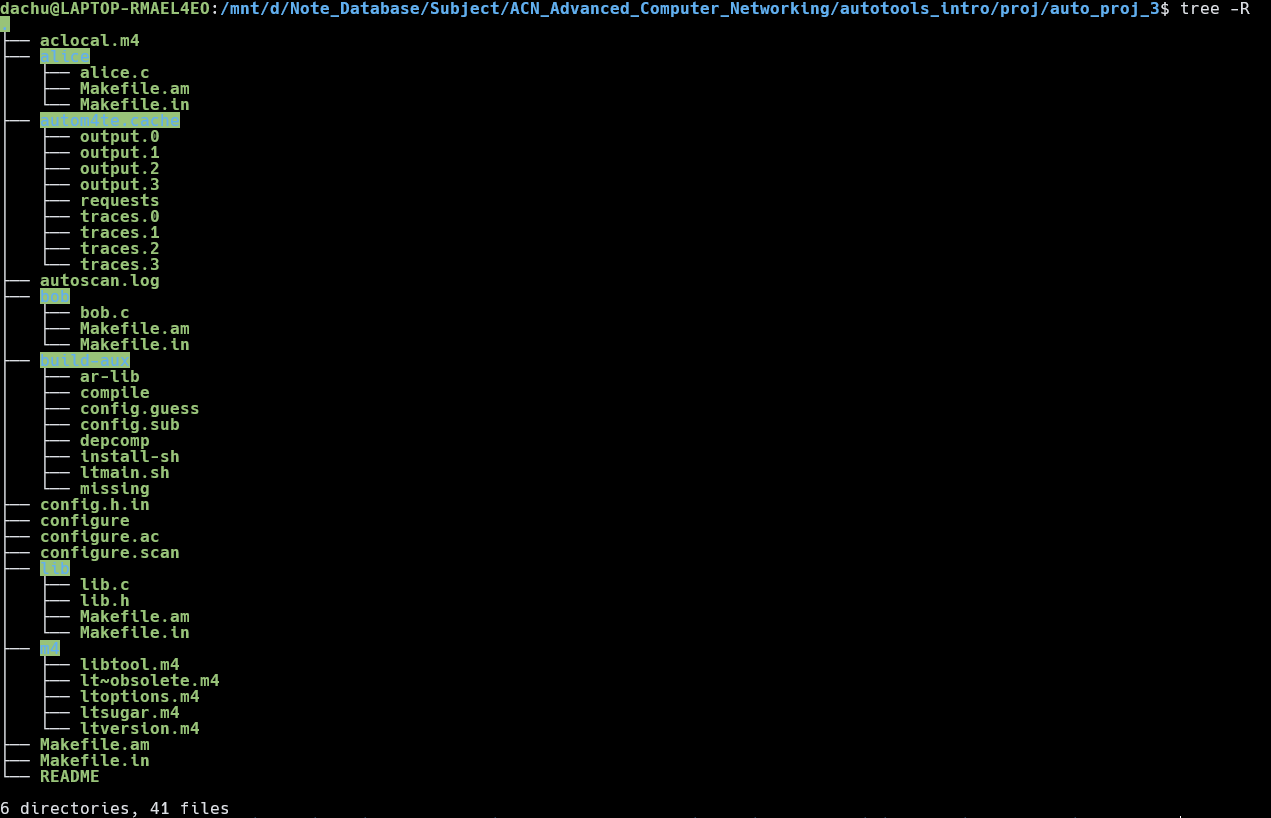
\includegraphics[width=0.8\textwidth]{../figure/autotool_13.png}
        \caption*{Tree structure after execution.}
    \end{figure}
\end{frame}

\section{Issues when compiling from sources}

\begin{frame}
    \frametitle{Compile from source process}

    After the distribution source is found, follows the following steps to compile.

    \begin{enumerate}
        \item Find installing steps in \alert{\texttt{readme.md}}, \alert{\texttt{README}}, or \alert{\texttt{INSTALL}}.
        \item If not, find \texttt{configure} to execute.
        \item If not, find custom installing scripts like \alert{\texttt{bootstrap}}, \alert{\texttt{autogen}} often in \textit{Bash} or \textit{Shell} syntax.
        \item If not, find corresponding configuration files of each build systems. If identified, use the convension compiling commands.
        \item In the build process, the build system might inform about missing dependency. Find the distribution source and repeat the process.
    \end{enumerate}
\end{frame}

\subsection{Distinguish build systems}

\begin{frame}
    \frametitle{Example: \texttt{pcre2}}

    \begin{center}
        \begin{tikzpicture}
            \node[anchor=south west,inner sep=0] at (0,0) {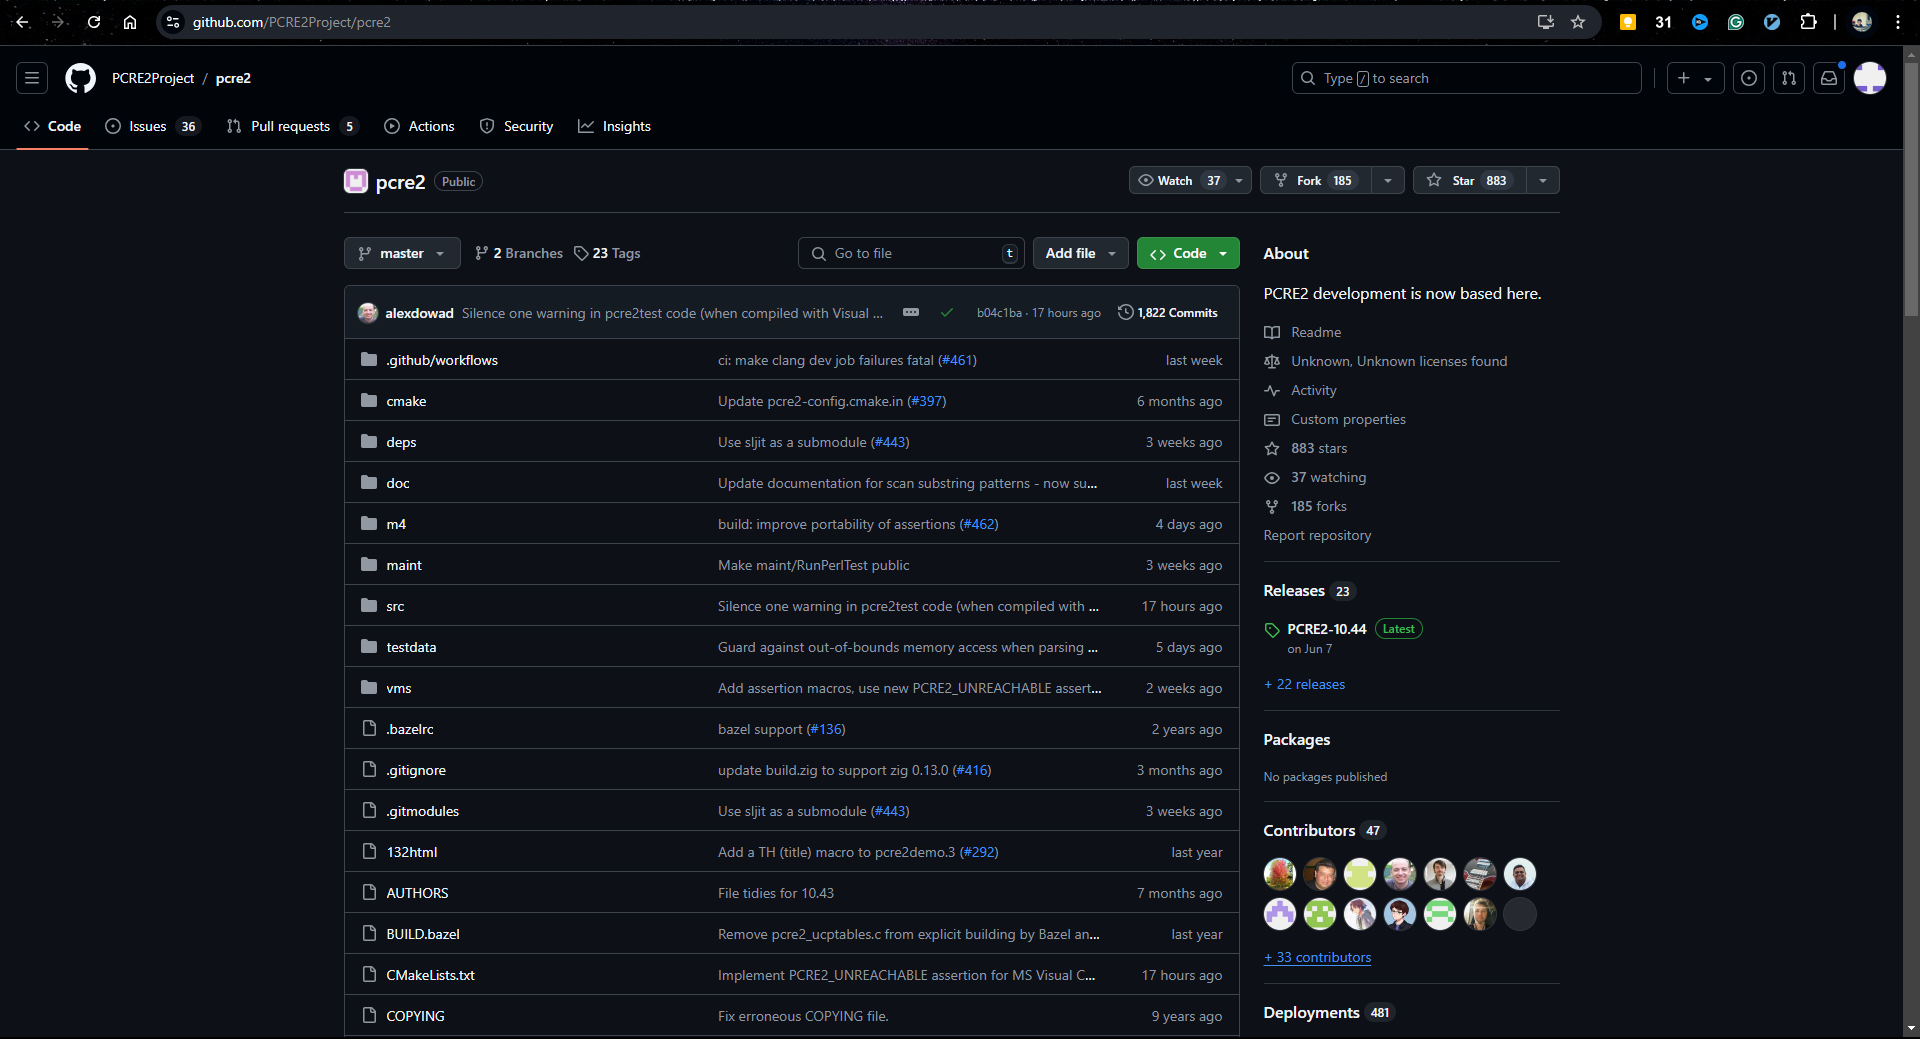
\includegraphics[width=\textwidth=0.8]{../figure/pcre2_1.png}};
            \draw[red,line width=0.1mm] (2.1,0.51) rectangle (7.9,0.3);
        \end{tikzpicture}
    \end{center}
\end{frame}

\begin{frame}
    \frametitle{Example: \texttt{pcre2}}

    \begin{center}
        \begin{tikzpicture}
            \node[anchor=south west,inner sep=0] at (0,0) {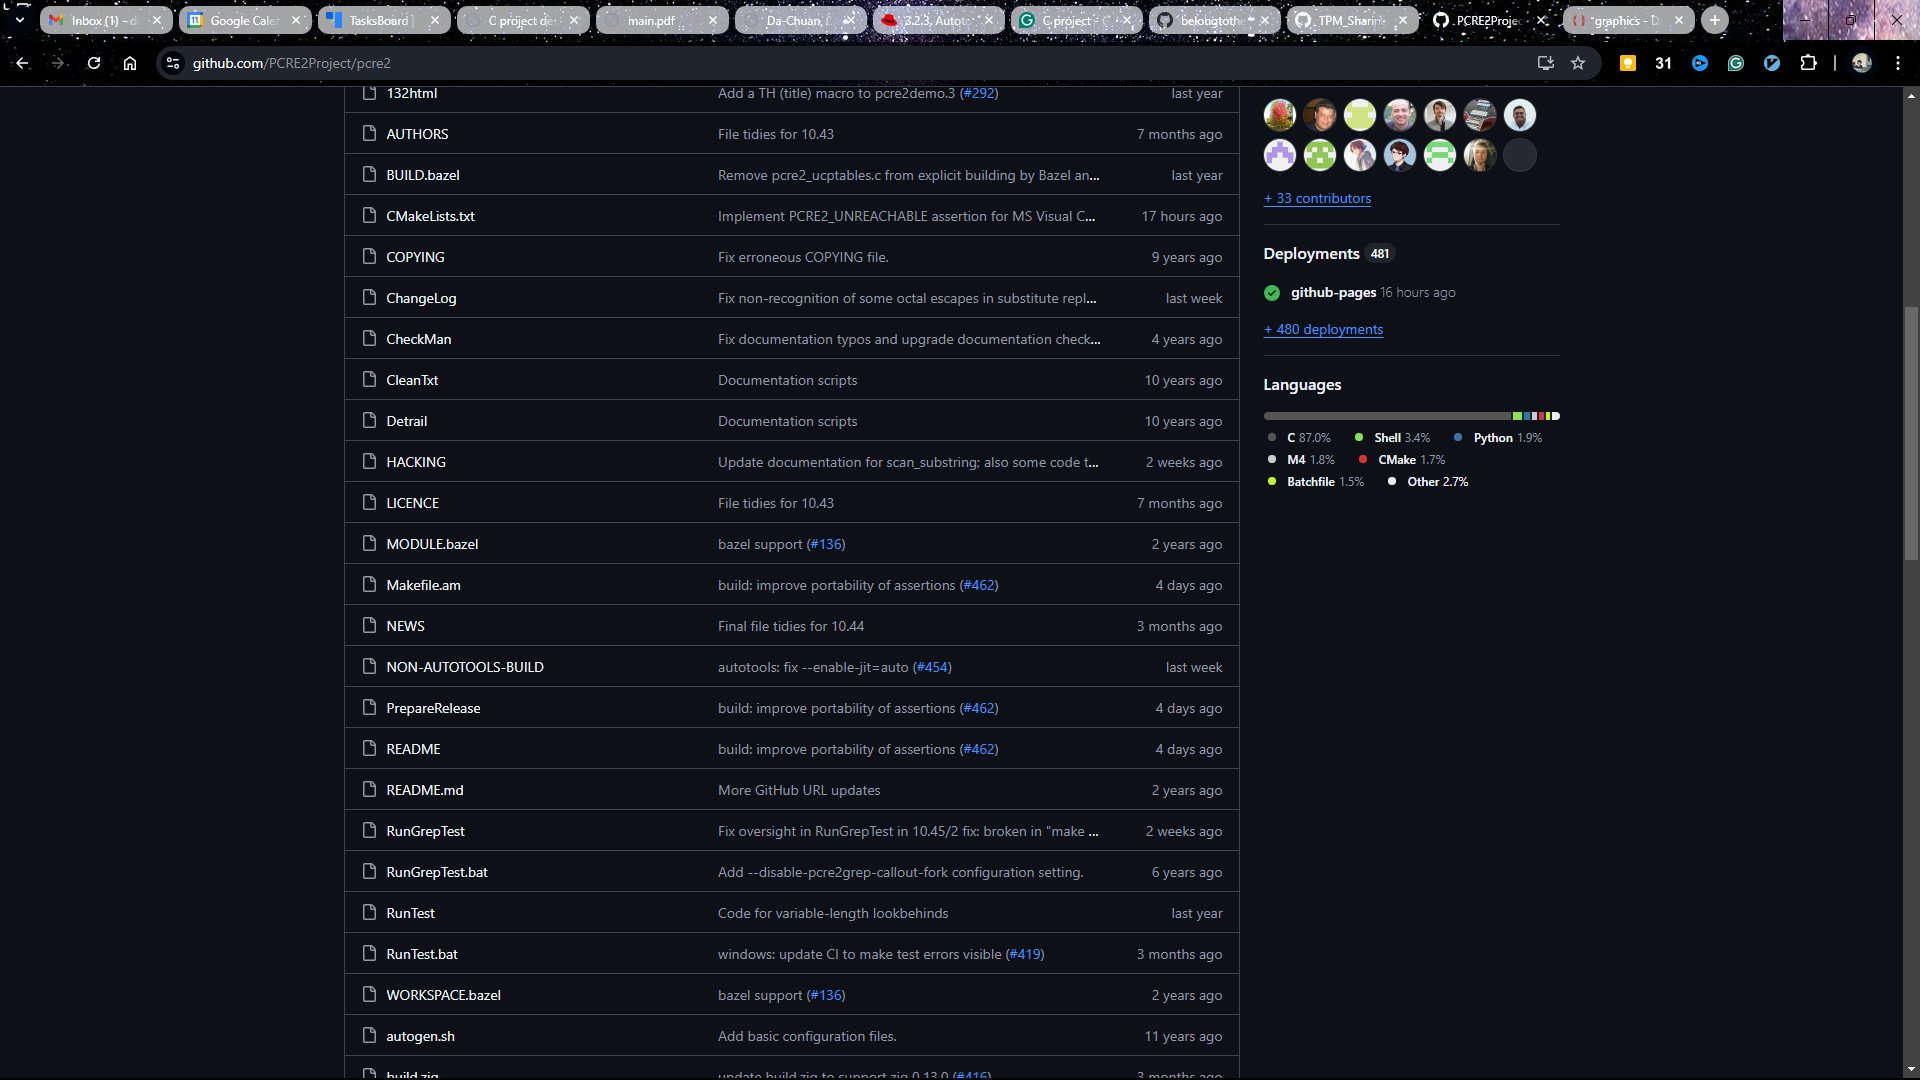
\includegraphics[width=\textwidth=0.8]{../figure/pcre2_2.png}};
            \draw[red,line width=0.1mm] (2.1,5.51) rectangle (7.9,5.3);
            \draw[red,line width=0.1mm] (2.1,3.21) rectangle (7.9,3.0);
            \draw[red,line width=0.1mm] (2.1,2.21) rectangle (7.9,2.0);
            \draw[red,line width=0.1mm] (2.1,1.93) rectangle (7.9,1.73);
            \draw[red,line width=0.1mm] (2.1,0.40) rectangle (7.9,0.20);
        \end{tikzpicture}
    \end{center}
\end{frame}

\begin{frame}
    \frametitle{Example: \texttt{pcre2}}

    \begin{center}
        \begin{tikzpicture}
            \node[anchor=south west,inner sep=0] at (0,0) {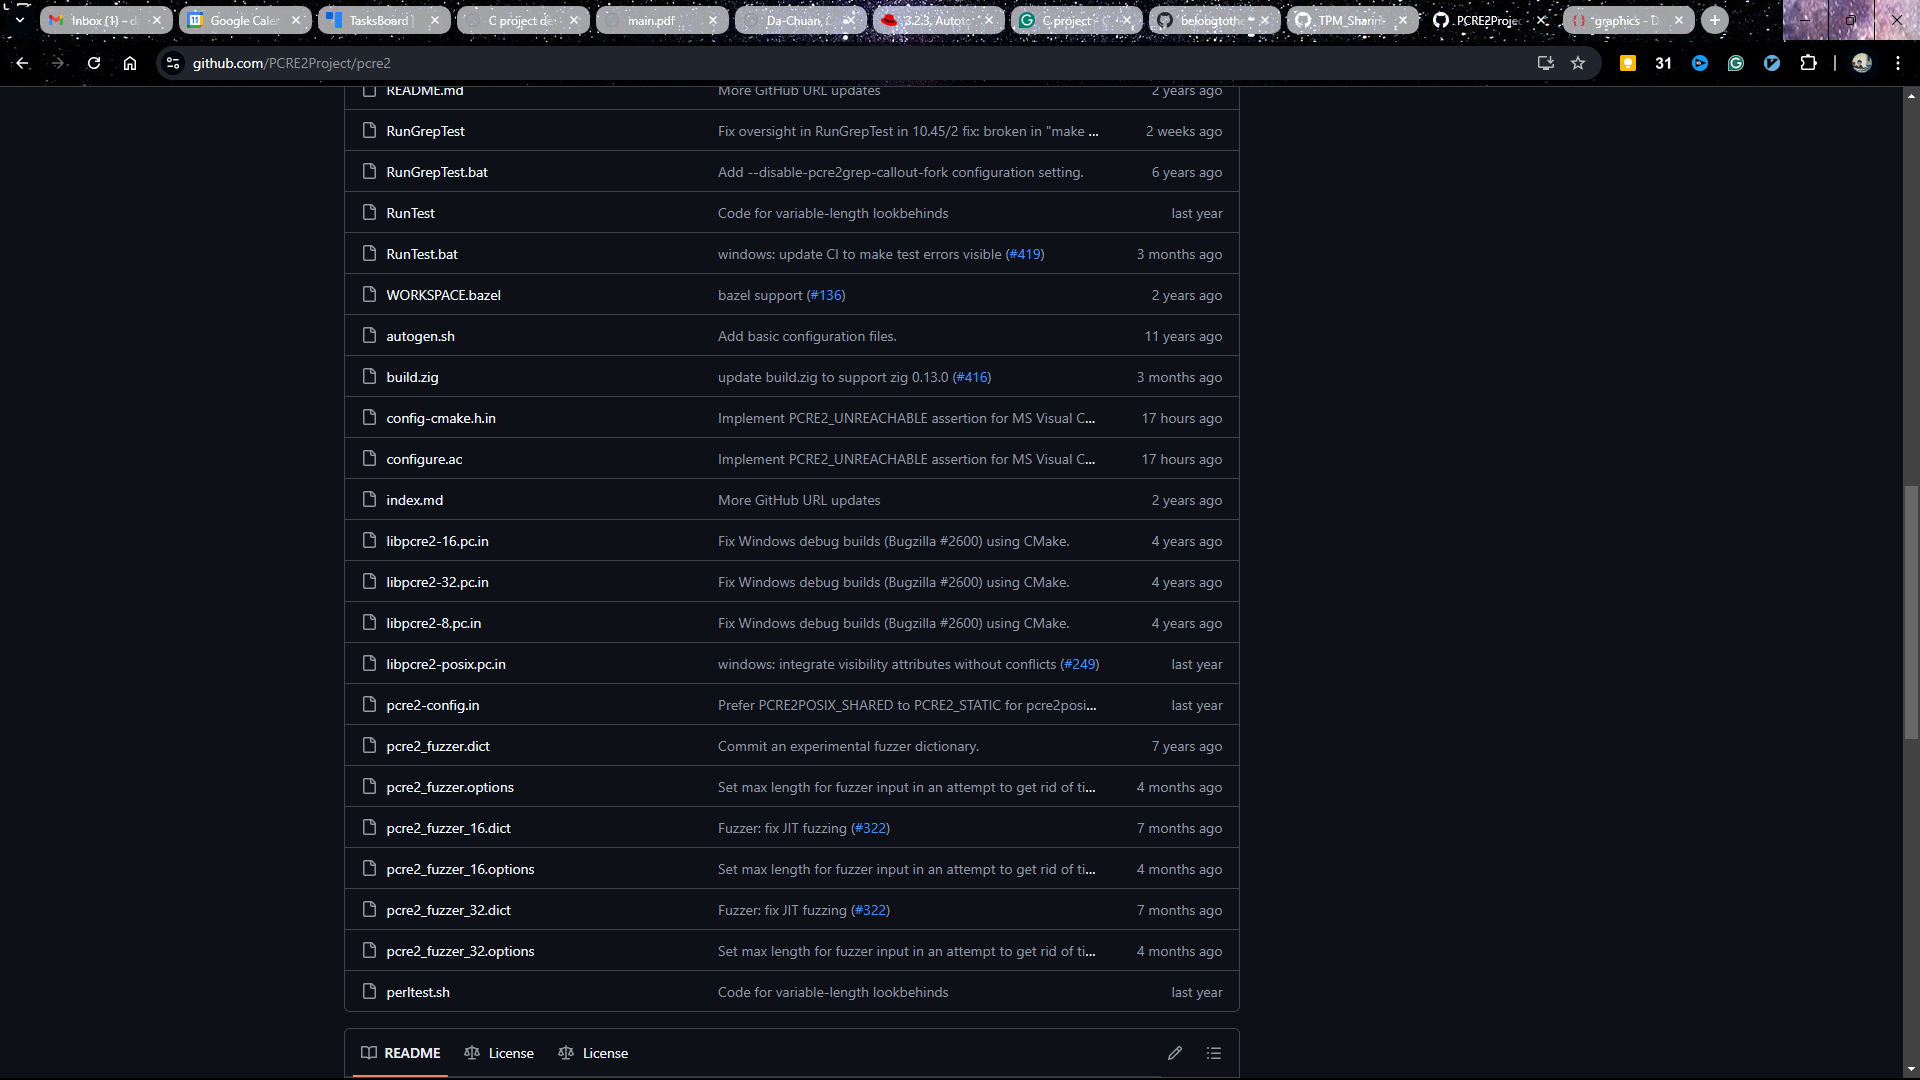
\includegraphics[width=\textwidth=0.8]{../figure/pcre2_3.png}};
            \draw[red,line width=0.1mm] (2.1,4.80) rectangle (7.9,4.60);
            \draw[red,line width=0.1mm] (2.1,4.00) rectangle (7.9,3.80);
        \end{tikzpicture}
    \end{center}
\end{frame}

\begin{frame}
    \frametitle{Example: \texttt{pcre2}}

    The above project structure is an example of source code distribution for development. Boxed files might not exist in the release version, and some new files might appear. Therefore, the same analysis on how to build the project should be done in the same way but after uncompressing the distributed software.

    The \texttt{pcre2} example should actually be compiled with the following commands:

    \begin{figure}[H]
        \centering
        \hfill
        \begin{minipage}{.8\textwidth}
            \inputminted[
                mathescape,
                linenos,
                autogobble,
                fontsize=\scriptsize,
            ]{bash}{E:\\GitHub\\presentation_in_LaTeX\\c_project_development\\script\\build_pcre2.sh}
        \end{minipage}
        \hfill
        \caption*{Code to compile lib \texttt{pcre2} with custom flags.}
    \end{figure}
\end{frame}

\begin{frame}
    \frametitle{Exercise: Build \texttt{pcre2}}

    Step 1: Find the distribution.

    \begin{figure}[H]
        \centering
        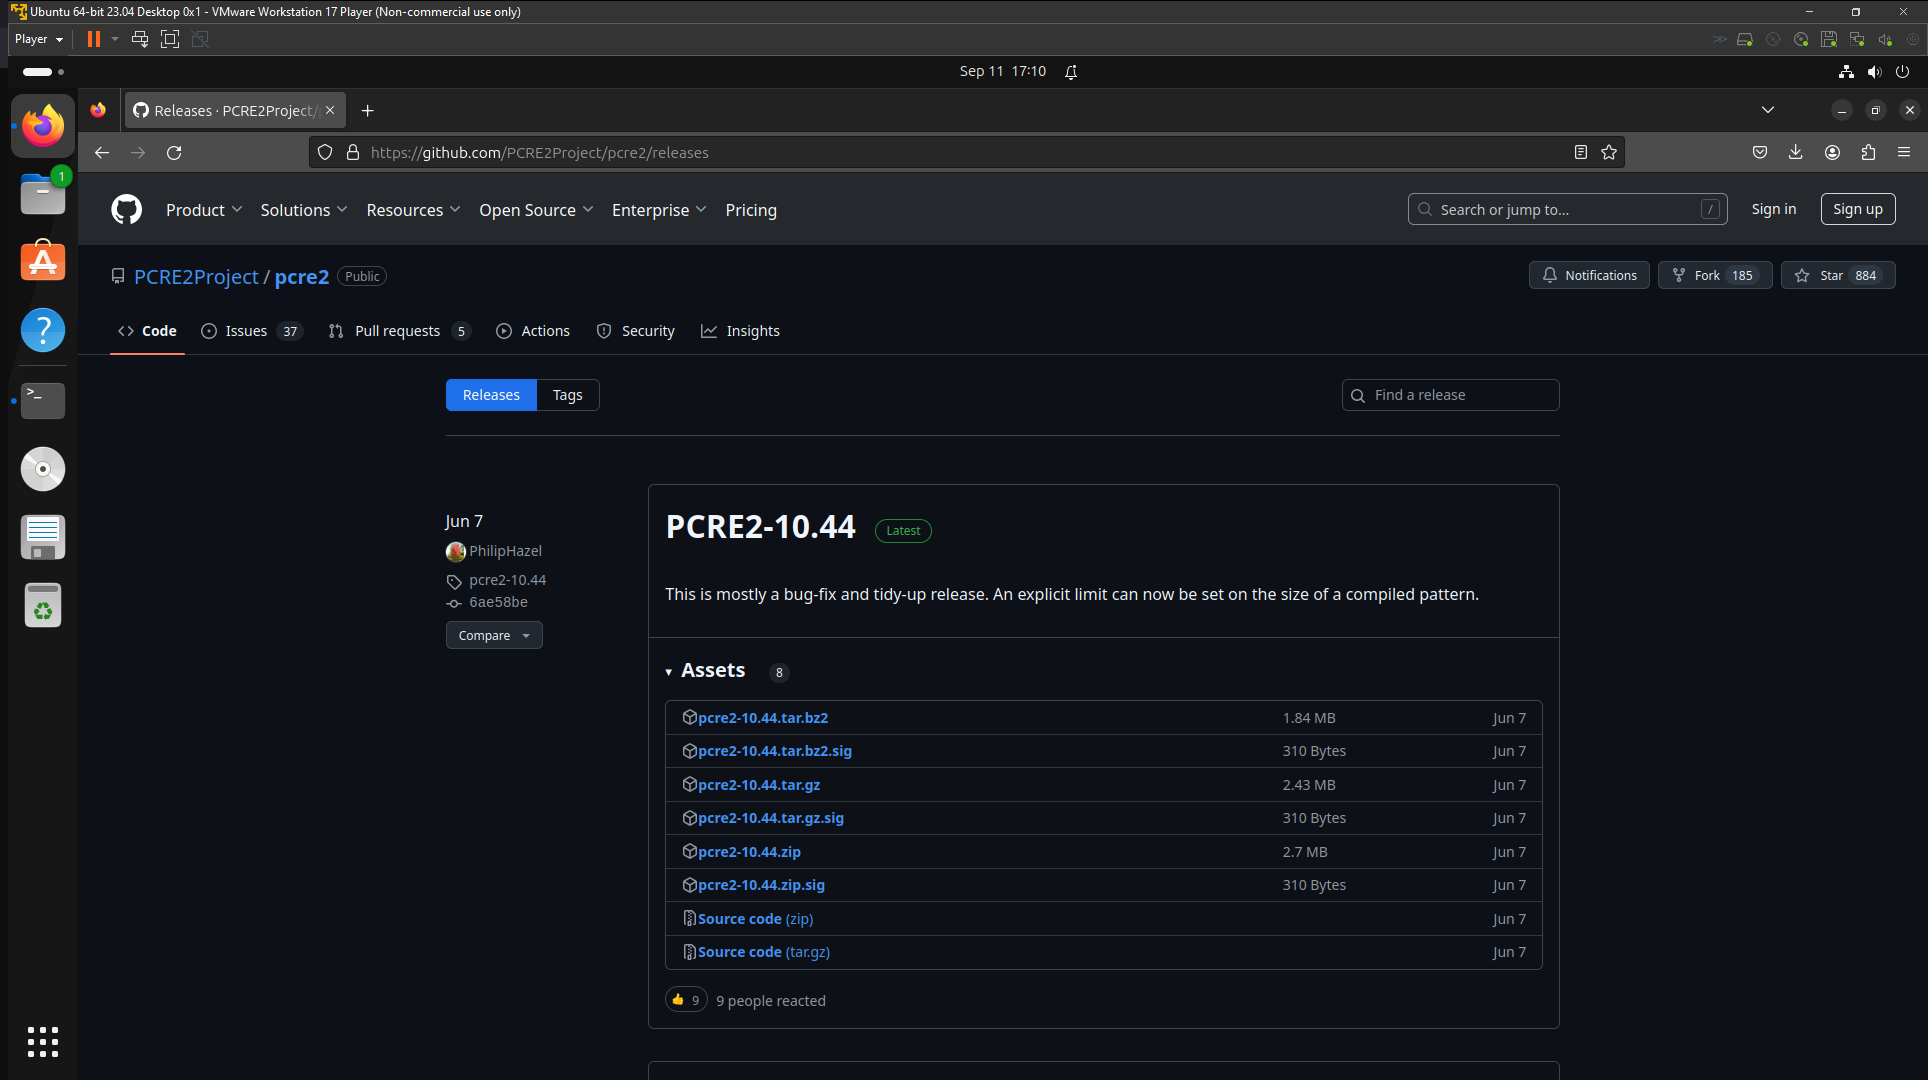
\includegraphics[width=0.9\textwidth]{../figure/pcre2_build_1.png}
    \end{figure}

\end{frame}

\begin{frame}
    \frametitle{Exercise: Build \texttt{pcre2}}

    Step 2: Copy the download link. (for downloading)

    \begin{figure}[H]
        \centering
        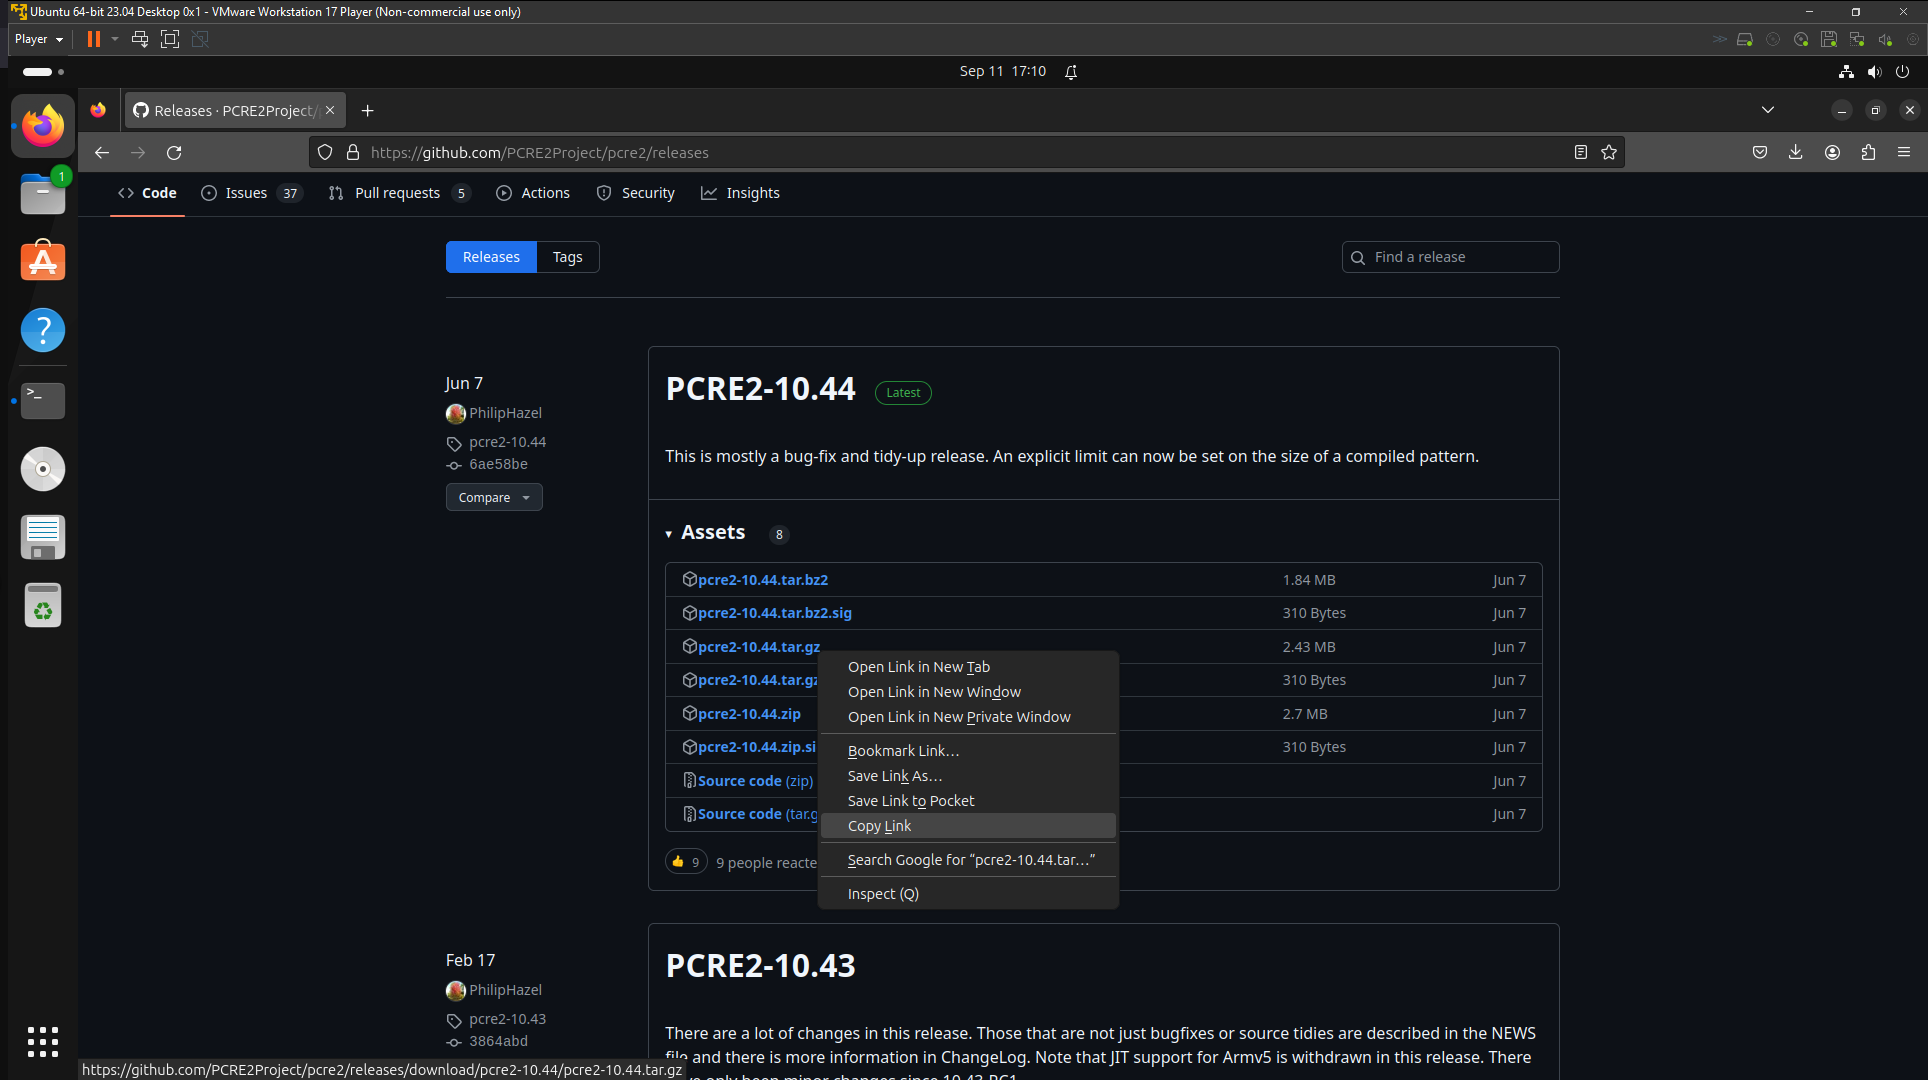
\includegraphics[width=0.9\textwidth]{../figure/pcre2_build_2.png}
    \end{figure}

\end{frame}

\begin{frame}
    \frametitle{Exercise: Build \texttt{pcre2}}

    Step 3: Download the compressed source code.

    \begin{figure}[H]
        \centering
        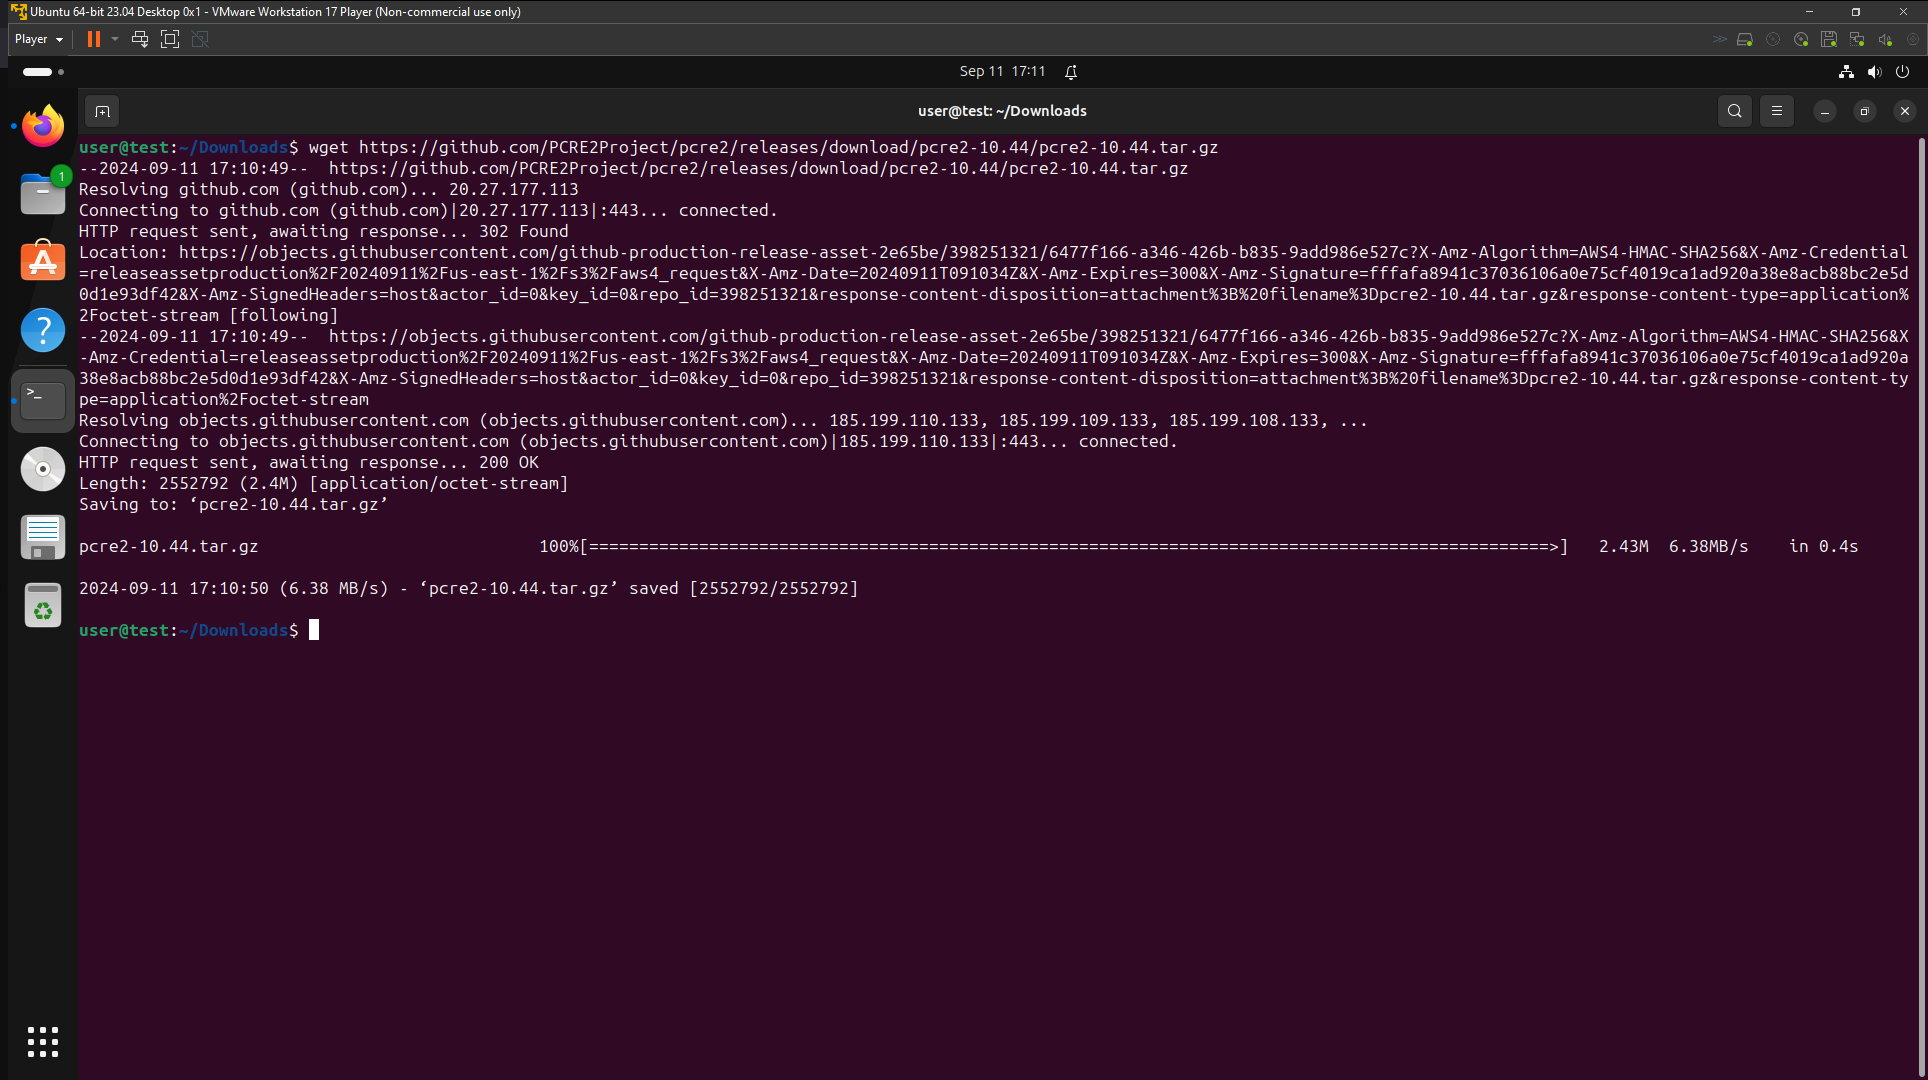
\includegraphics[width=0.9\textwidth]{../figure/pcre2_build_3.png}
    \end{figure}

\end{frame}

\begin{frame}
    \frametitle{Exercise: Build \texttt{pcre2}}

    Step 4: Create a directory with custom naming and uncompress the source code into it. Notice that there are binary \alert{\texttt{./configure}} existed, and can be used for building.

    \begin{figure}[H]
        \centering
        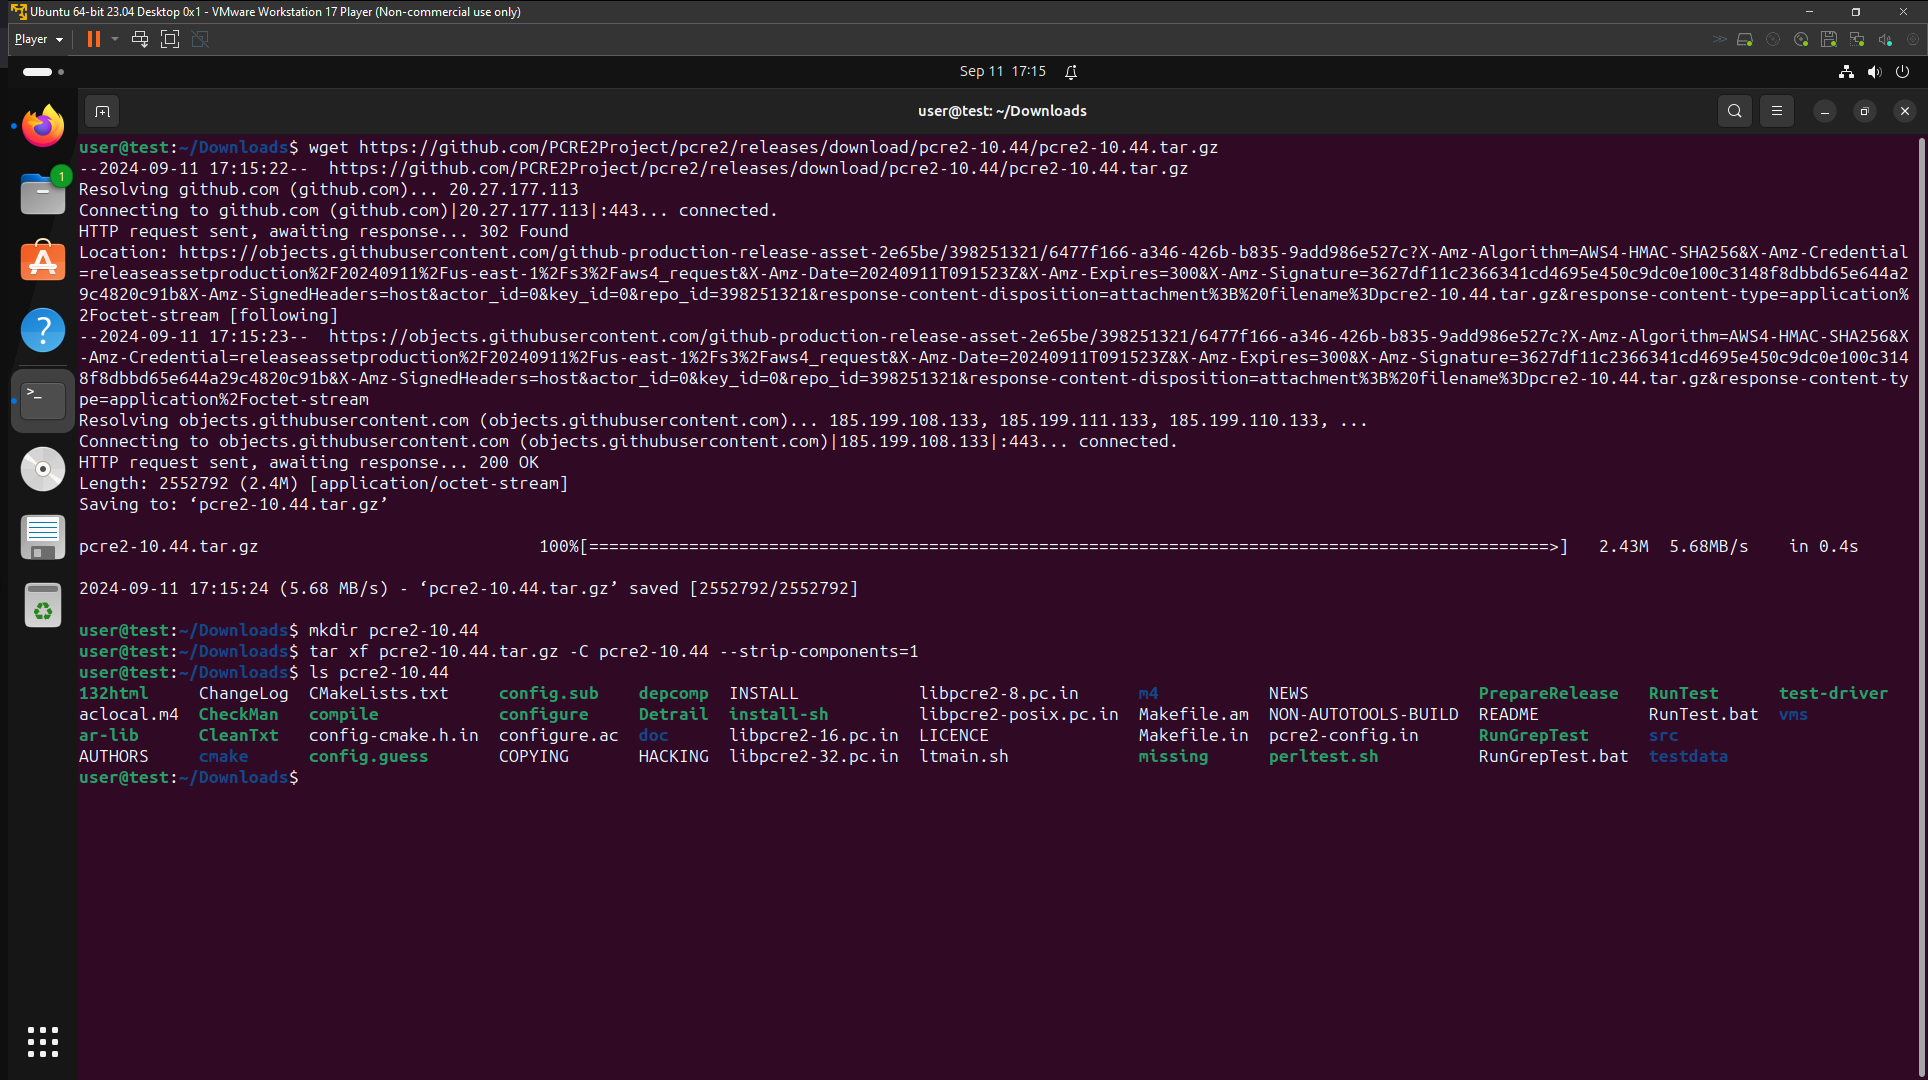
\includegraphics[width=0.9\textwidth]{../figure/pcre2_build_4.png}
    \end{figure}

\end{frame}

\begin{frame}
    \frametitle{Exercise: Build \texttt{pcre2}}

    Step 5: Execute \texttt{./configure} to configure files for building.

    \begin{figure}[H]
        \centering
        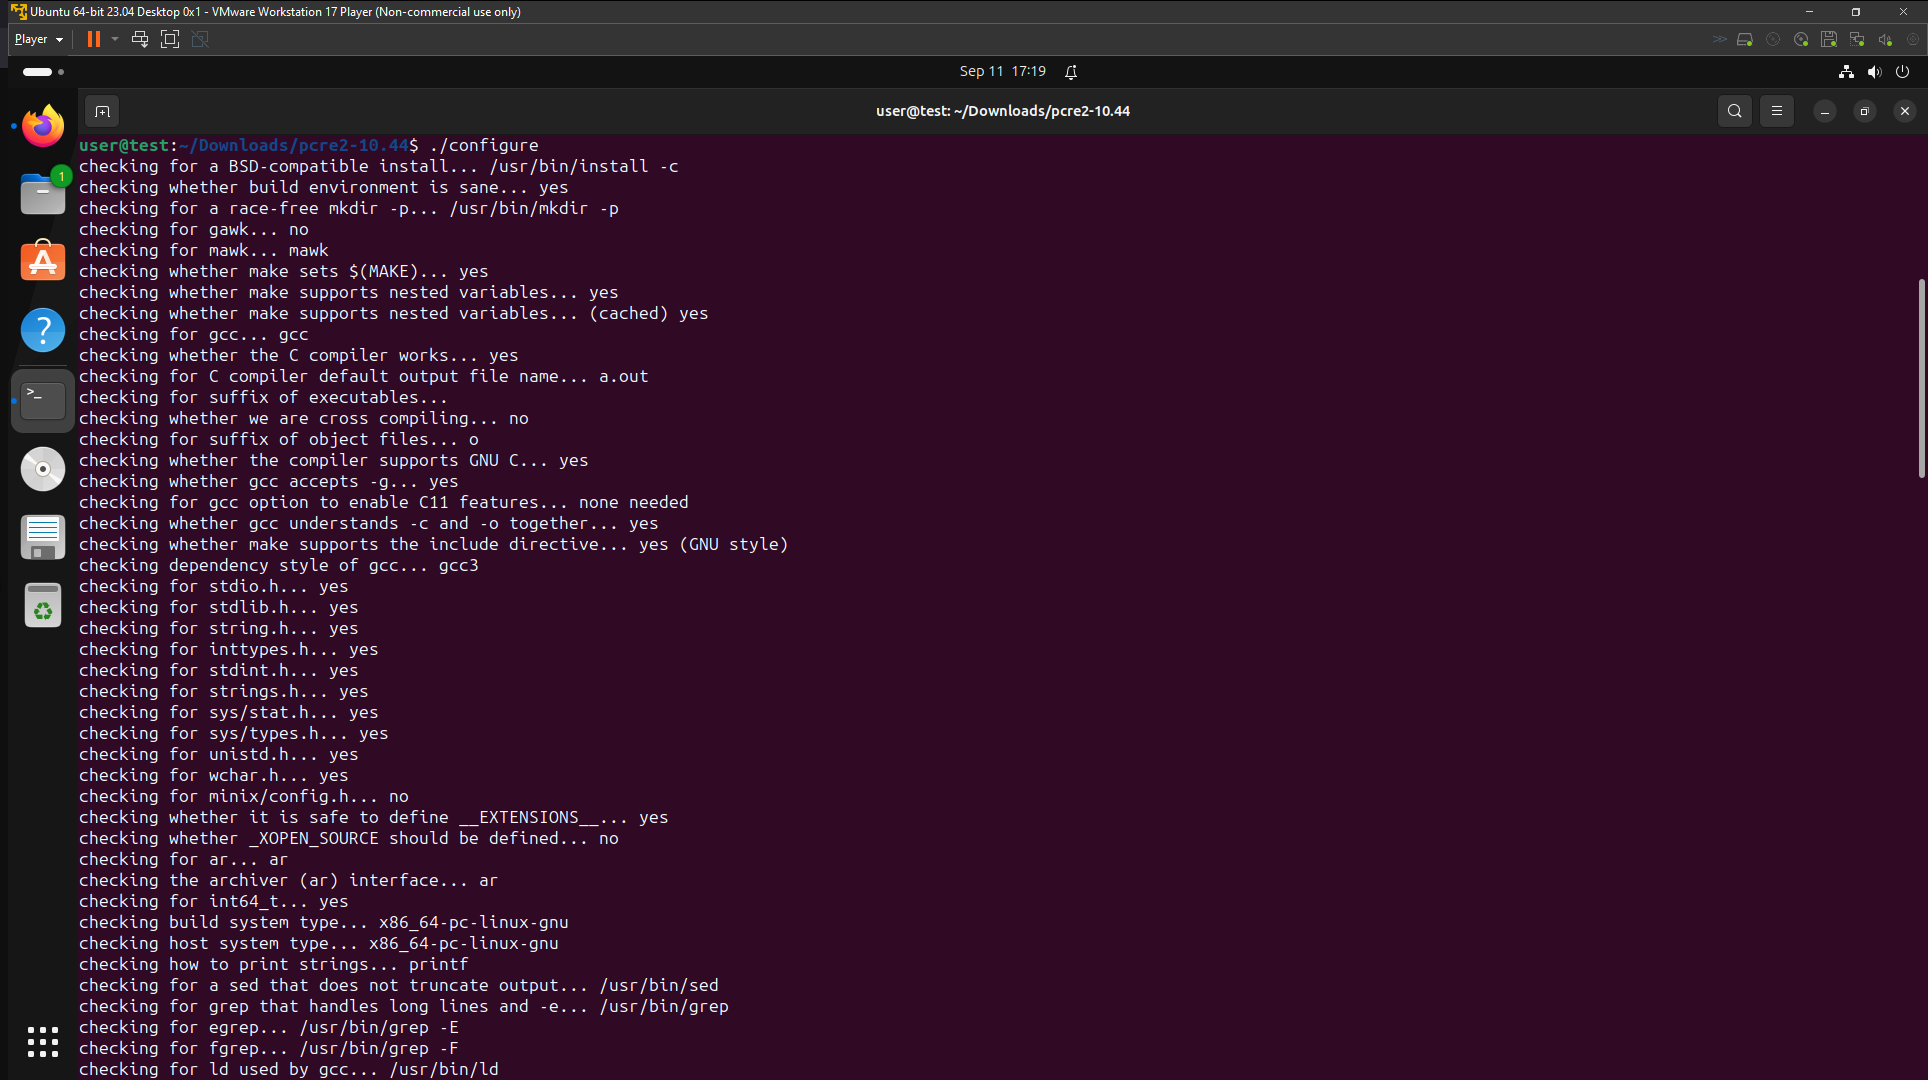
\includegraphics[width=0.9\textwidth]{../figure/pcre2_build_5.png}
    \end{figure}

\end{frame}

\begin{frame}
    \frametitle{Exercise: Build \texttt{pcre2}}

    Step 6: Make sure no error is shown in the output and execute \texttt{make} to build

    \begin{figure}[H]
        \centering
        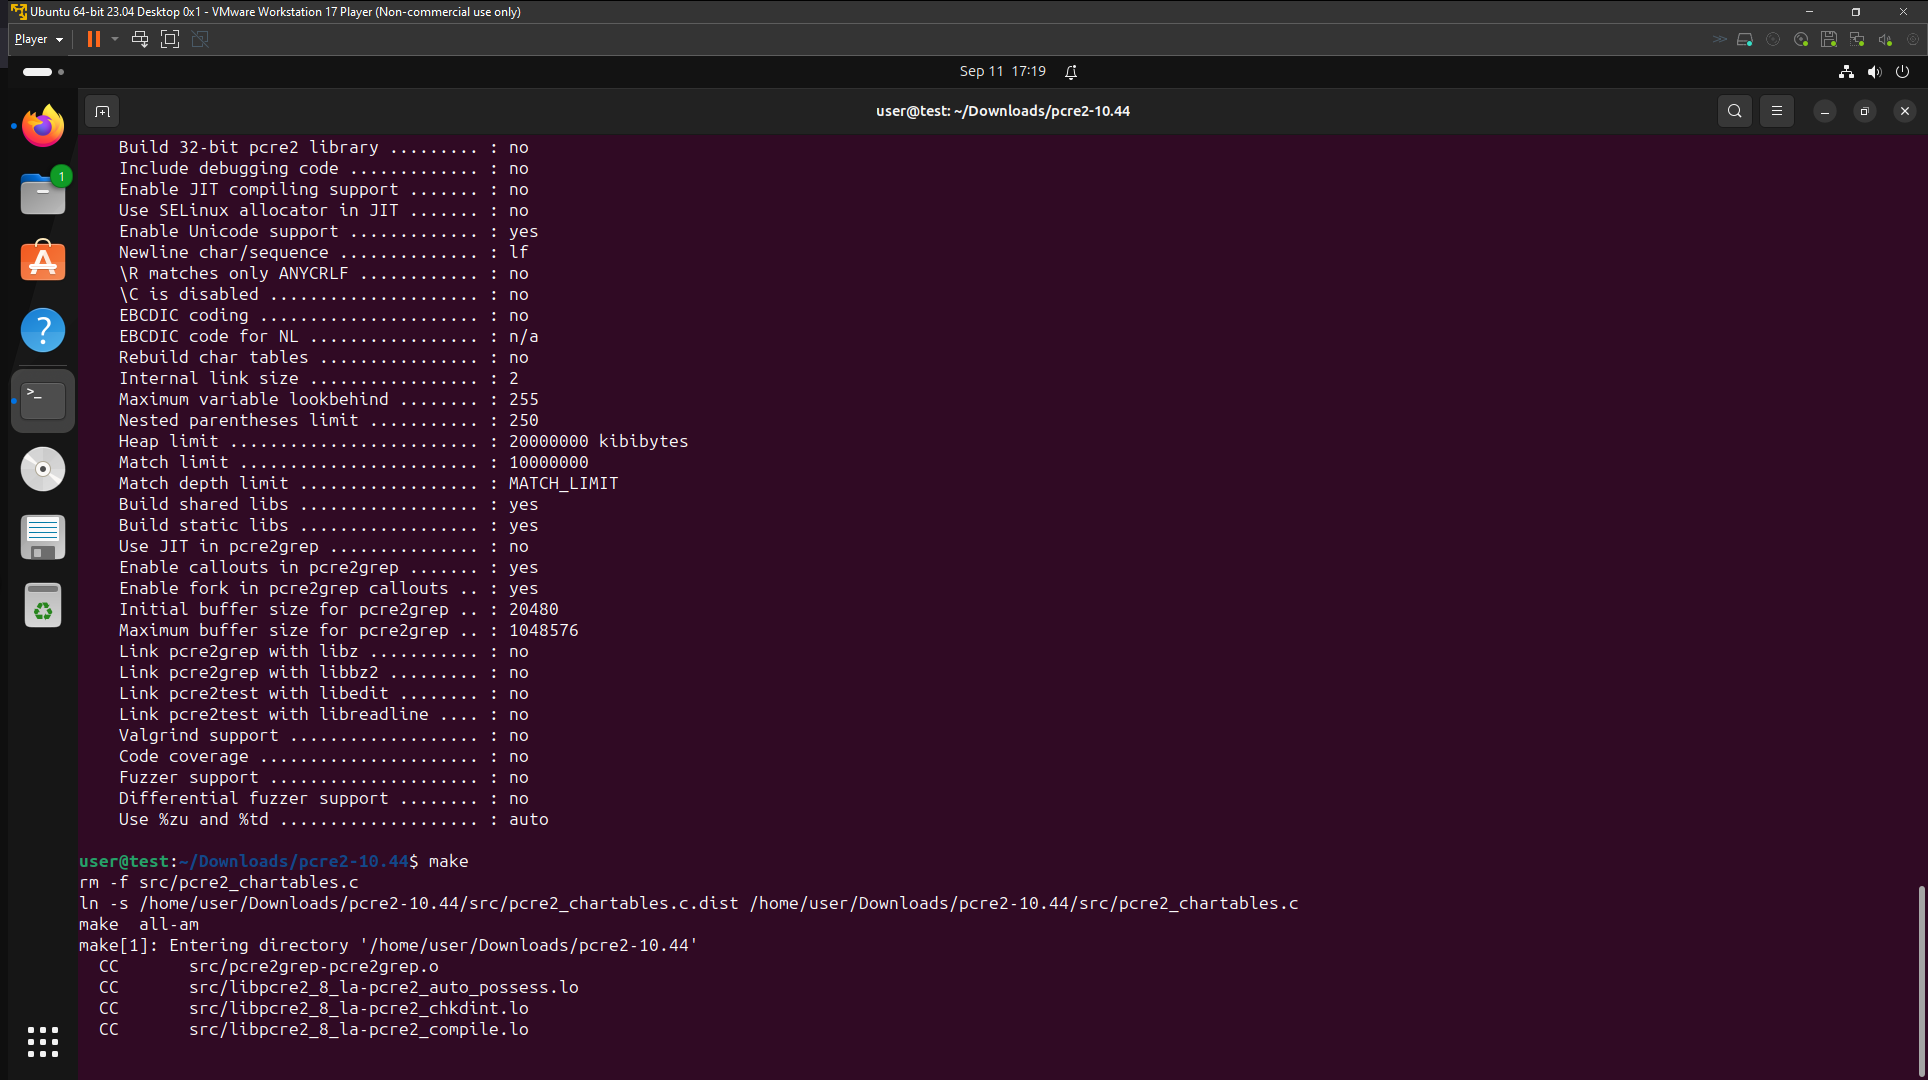
\includegraphics[width=0.9\textwidth]{../figure/pcre2_build_6.png}
    \end{figure}

\end{frame}

\begin{frame}
    \frametitle{Exercise: Build \texttt{pcre2}}

    \begin{figure}[H]
        \centering
        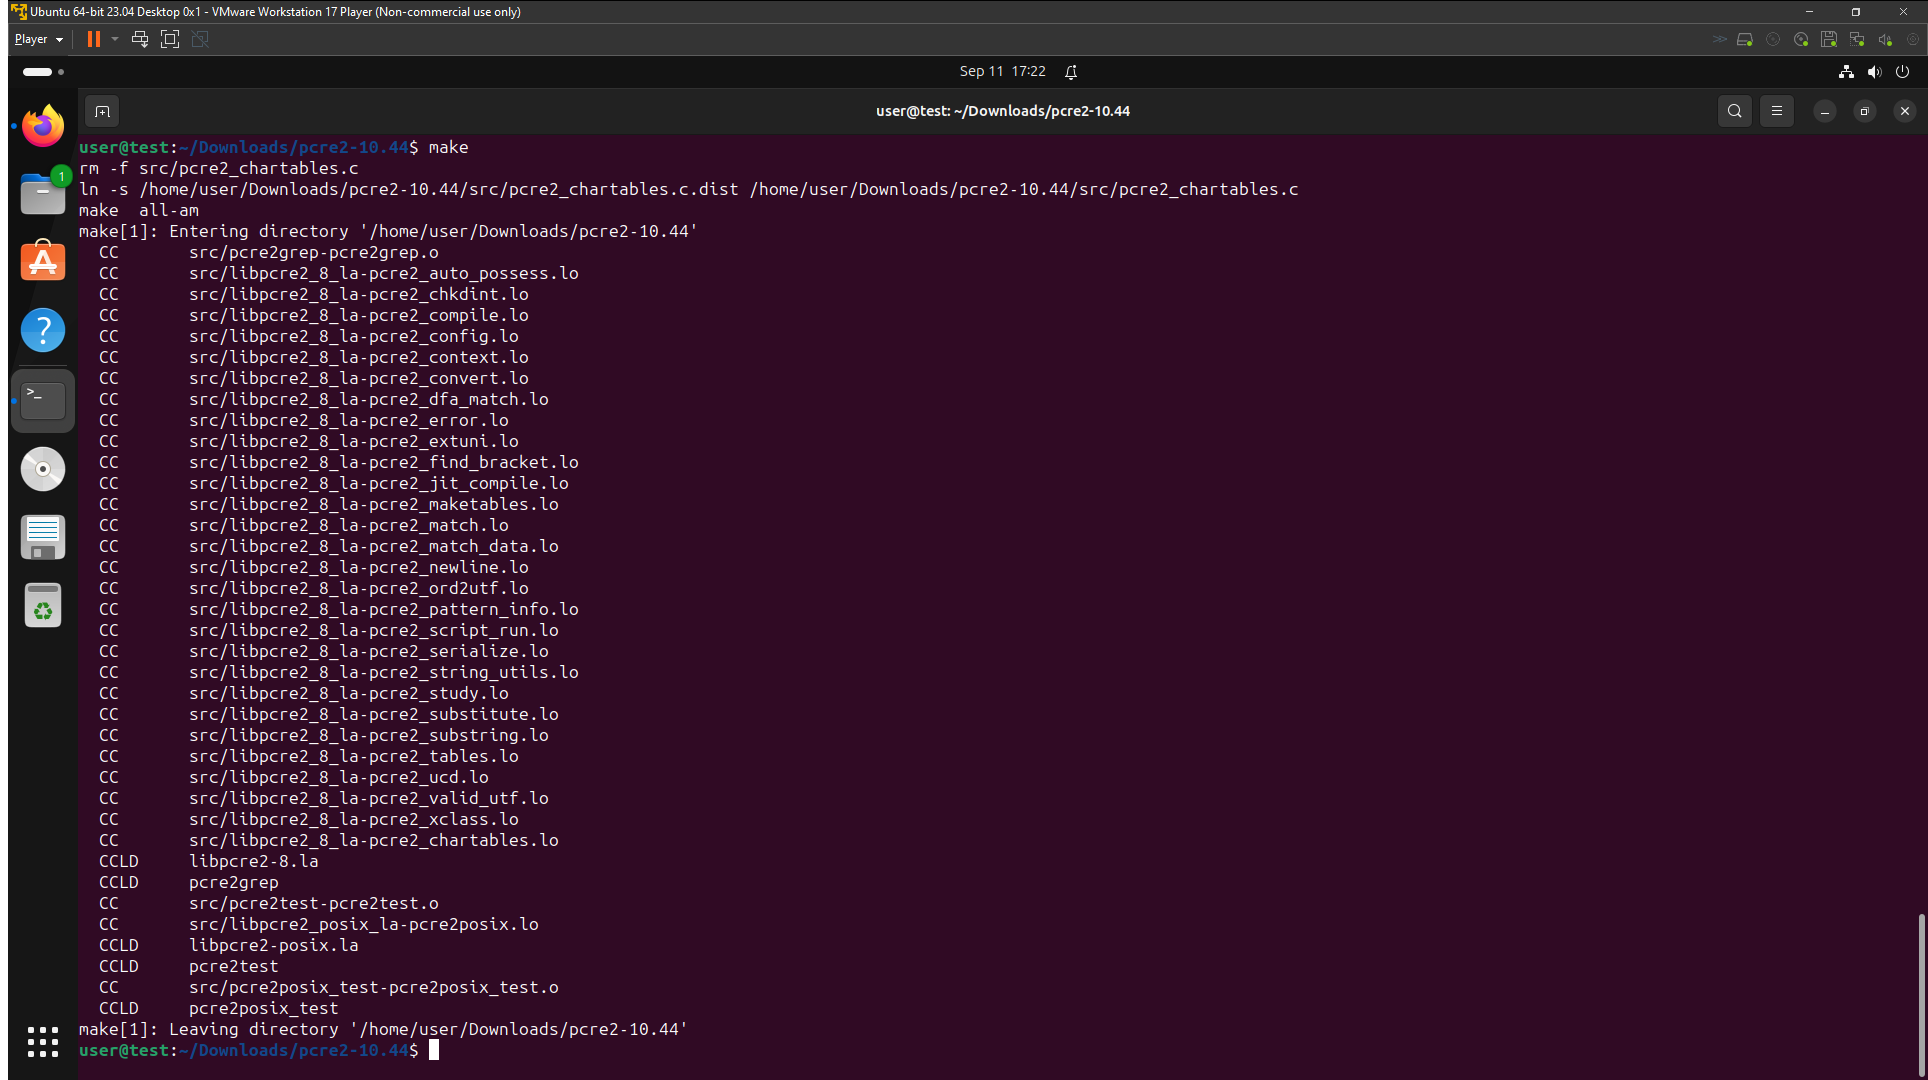
\includegraphics[width=0.9\textwidth]{../figure/pcre2_build_7.png}
        \caption*{Result of building \texttt{pcre2}.}
    \end{figure}

\end{frame}

\subsection{Resolve dependency issue}

\begin{frame}
    \frametitle{Exercise: Build \texttt{json-c}}

    Step 1: Download, uncompress, and examine the content of the project.

    \begin{figure}[H]
        \centering
        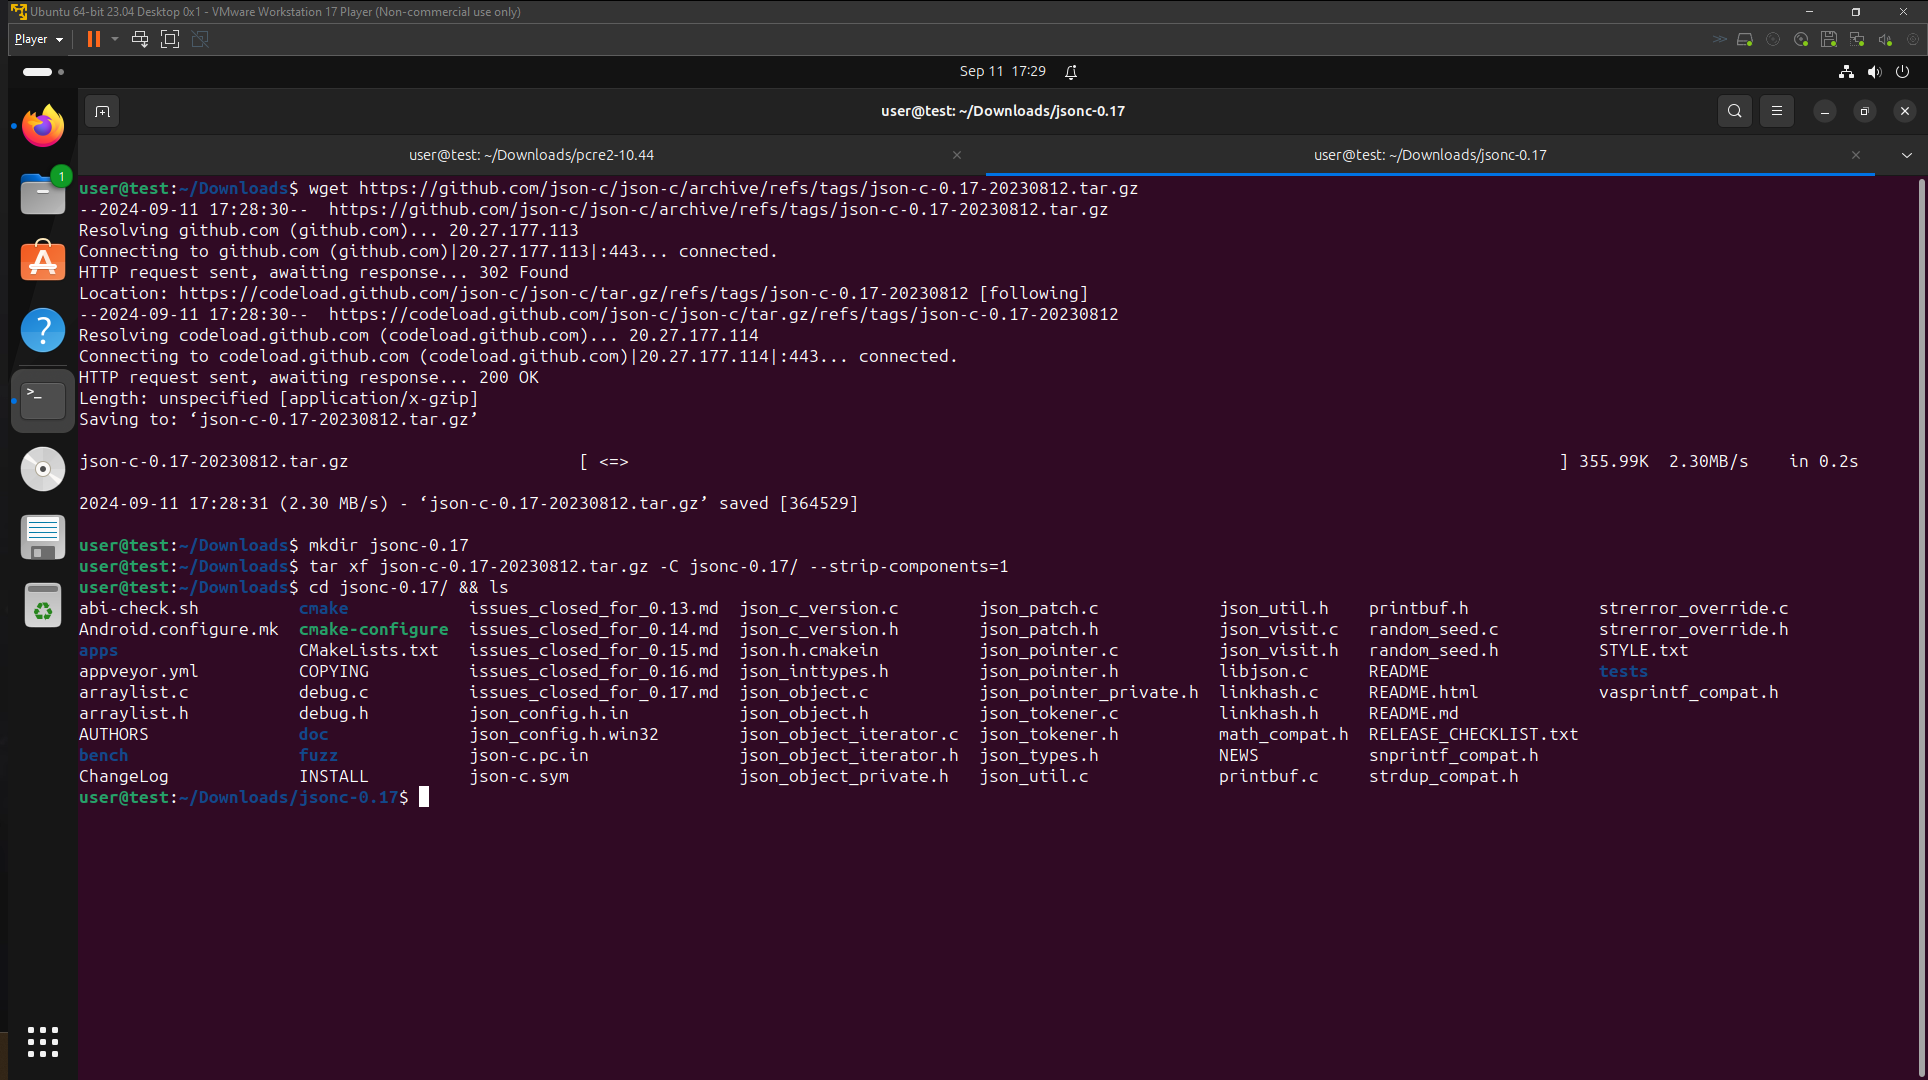
\includegraphics[width=0.9\textwidth]{../figure/jsonc_build_1.png}
    \end{figure}
\end{frame}

\begin{frame}
    \frametitle{Exercise: Build \texttt{json-c}}

    Step 2: Check \texttt{INSTALL} and \texttt{README.md} for installation steps.

    \begin{figure}[H]
        \centering
        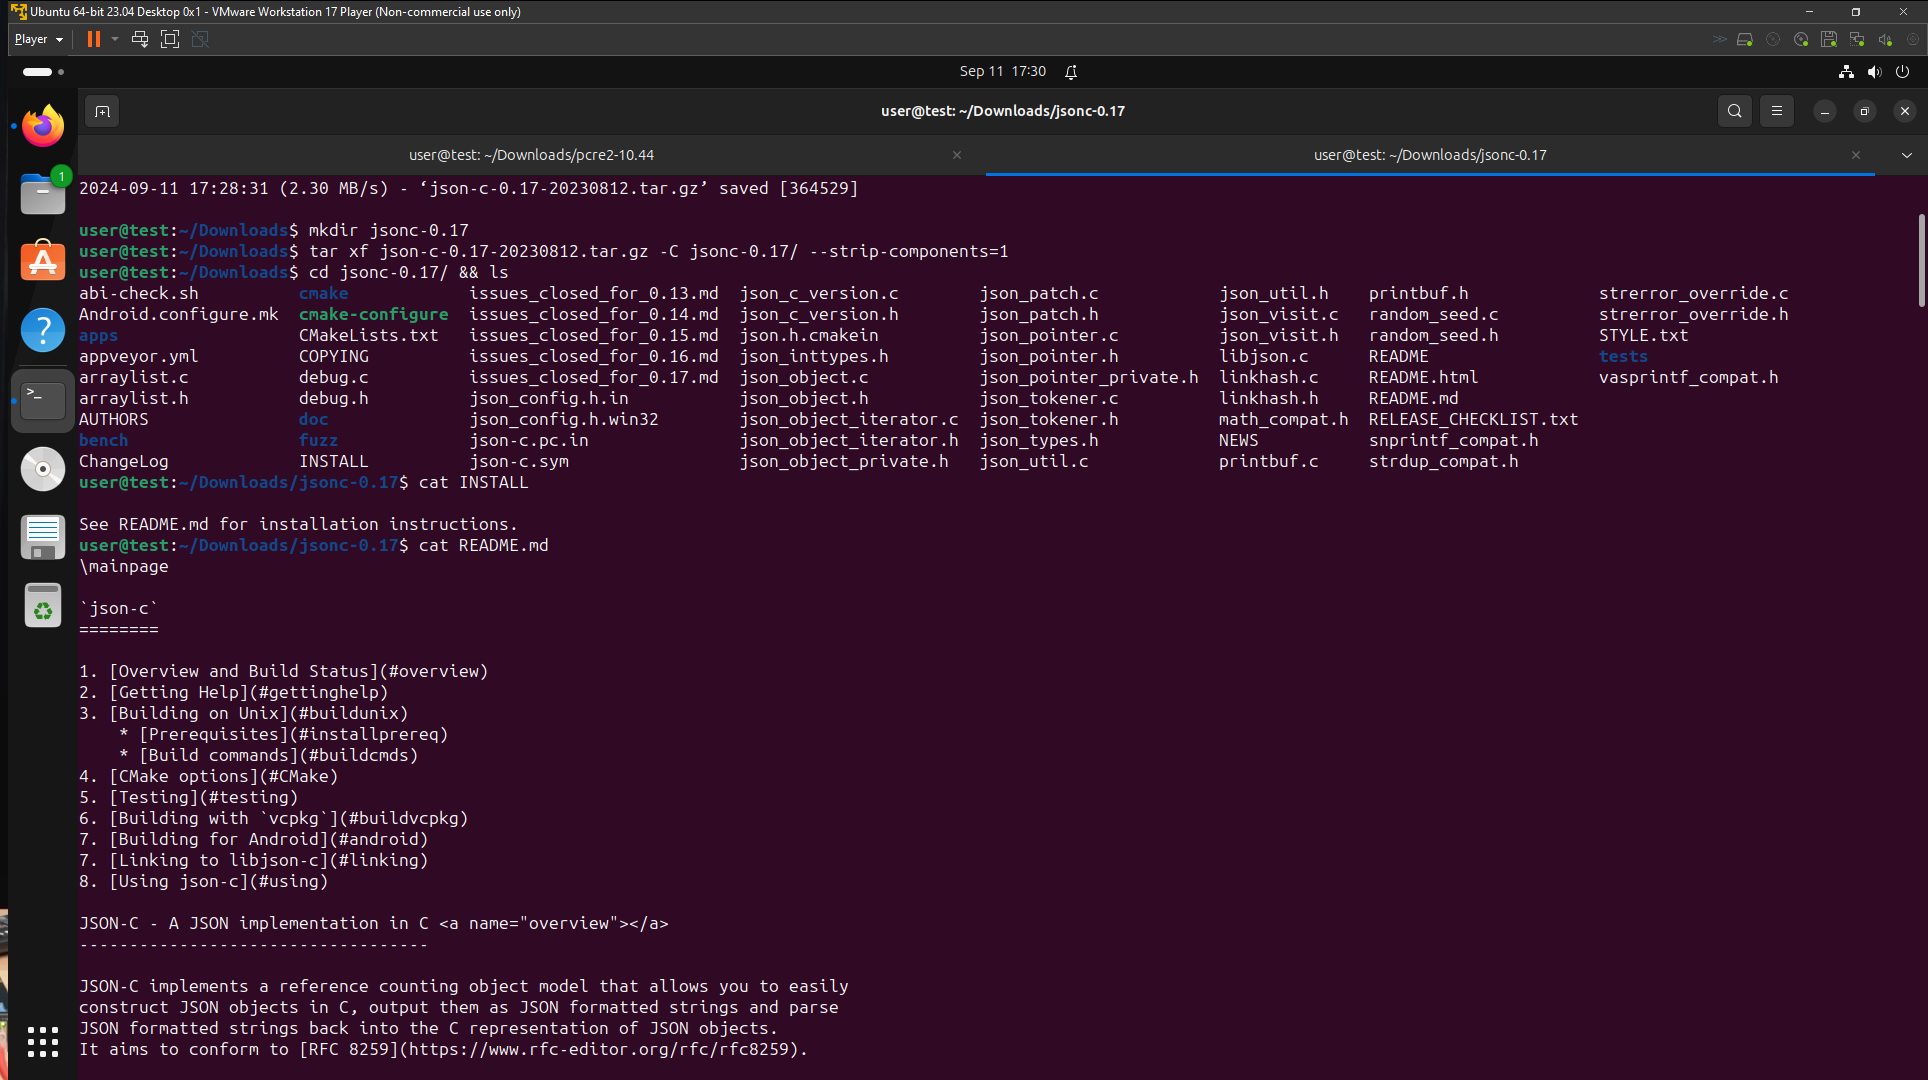
\includegraphics[width=0.9\textwidth]{../figure/jsonc_build_2.png}
    \end{figure}
\end{frame}

\begin{frame}
    \frametitle{Exercise: Build \texttt{json-c}}

    Step 3: Locate official installation steps.

    \begin{figure}[H]
        \centering
        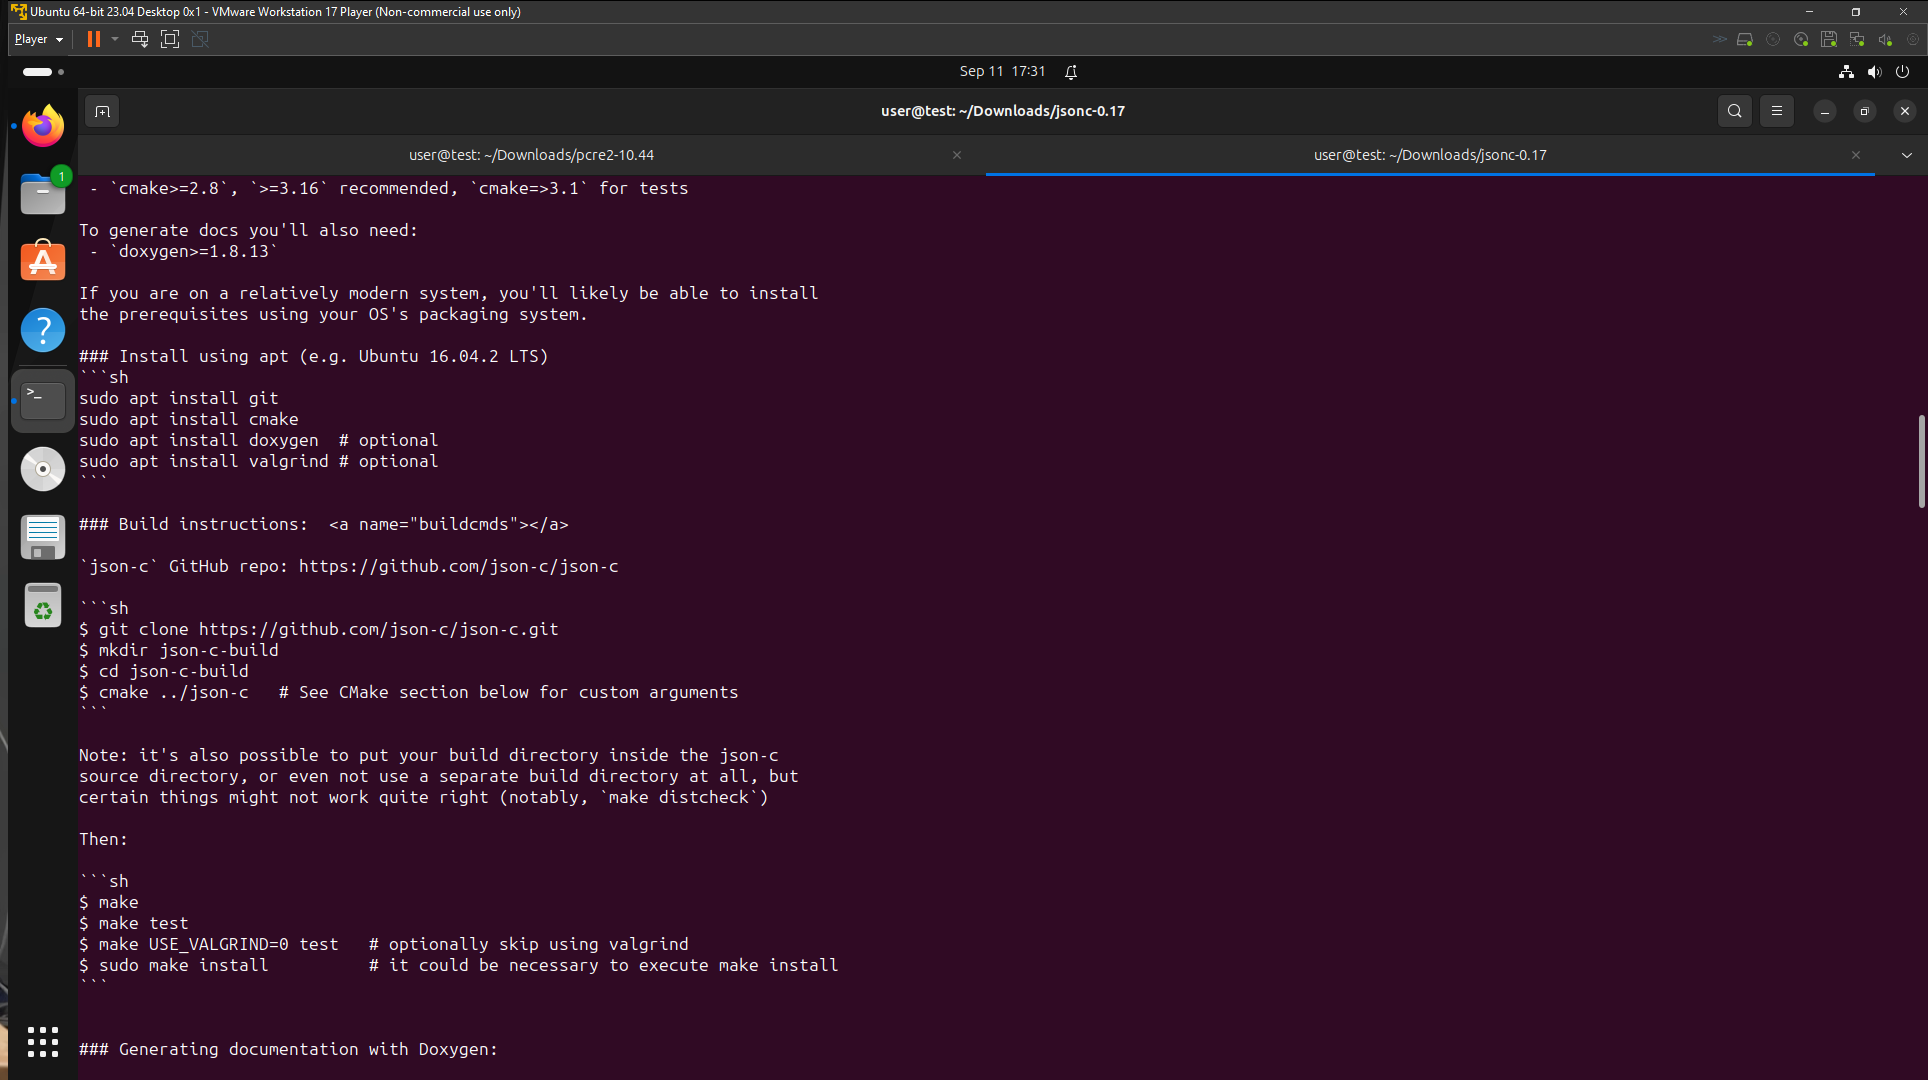
\includegraphics[width=0.9\textwidth]{../figure/jsonc_build_3.png}
    \end{figure}
\end{frame}

\begin{frame}
    \frametitle{Exercise: Build \texttt{json-c}}

    Step 4: Follows the installation steps.

    \begin{figure}[H]
        \centering
        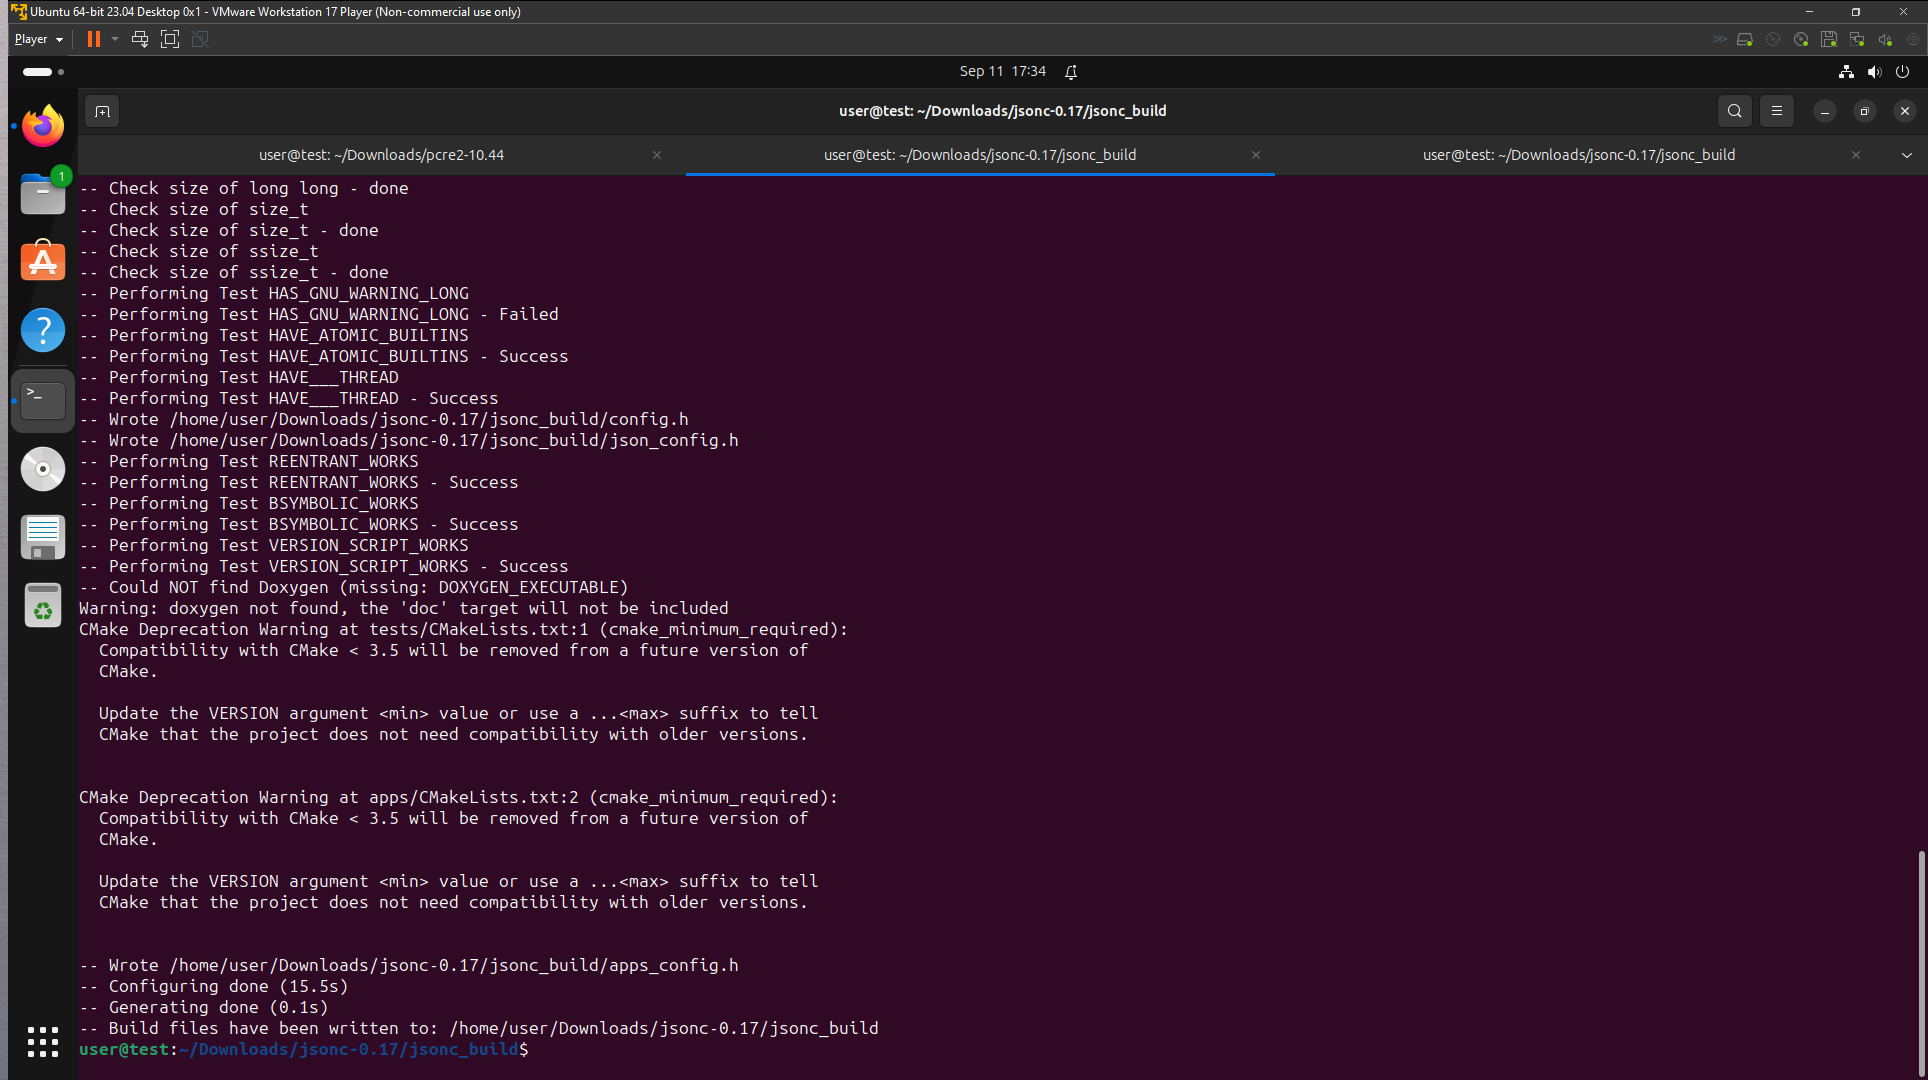
\includegraphics[width=0.9\textwidth]{../figure/jsonc_build_4.png}
        \caption*{Executed \texttt{mkdir jsonc\_build \&\& cd json\_cbuild \&\& cmake ..}}
    \end{figure}
\end{frame}

\begin{frame}
    \frametitle{Exercise: Build \texttt{json-c}}

    Notice there are two warnings indicating dependency issues. 

    \begin{itemize}
        \item \alert{\texttt{doxygen not found}}: Find the distribution of doxygen and install it.
        \item \alert{\texttt{CMake deprecation}}: Update CMake version or compile CMake from source for the latest version.
    \end{itemize}

    These kinds of problems can appear frequently. But make sure to check whether the corresponding \texttt{*.pc} files of dependency exists in default location. Sometimes the build system will not install the \texttt{*.pc} files (especially Meson), making other build systems cannot find the required dependency with \alert{\texttt{pkg-config}}.
\end{frame}

\begin{frame}
    \frametitle{Exercise: Build \texttt{json-c}}

    Step 5: Build the project. (The warnings are skipped)

    \begin{figure}[H]
        \centering
        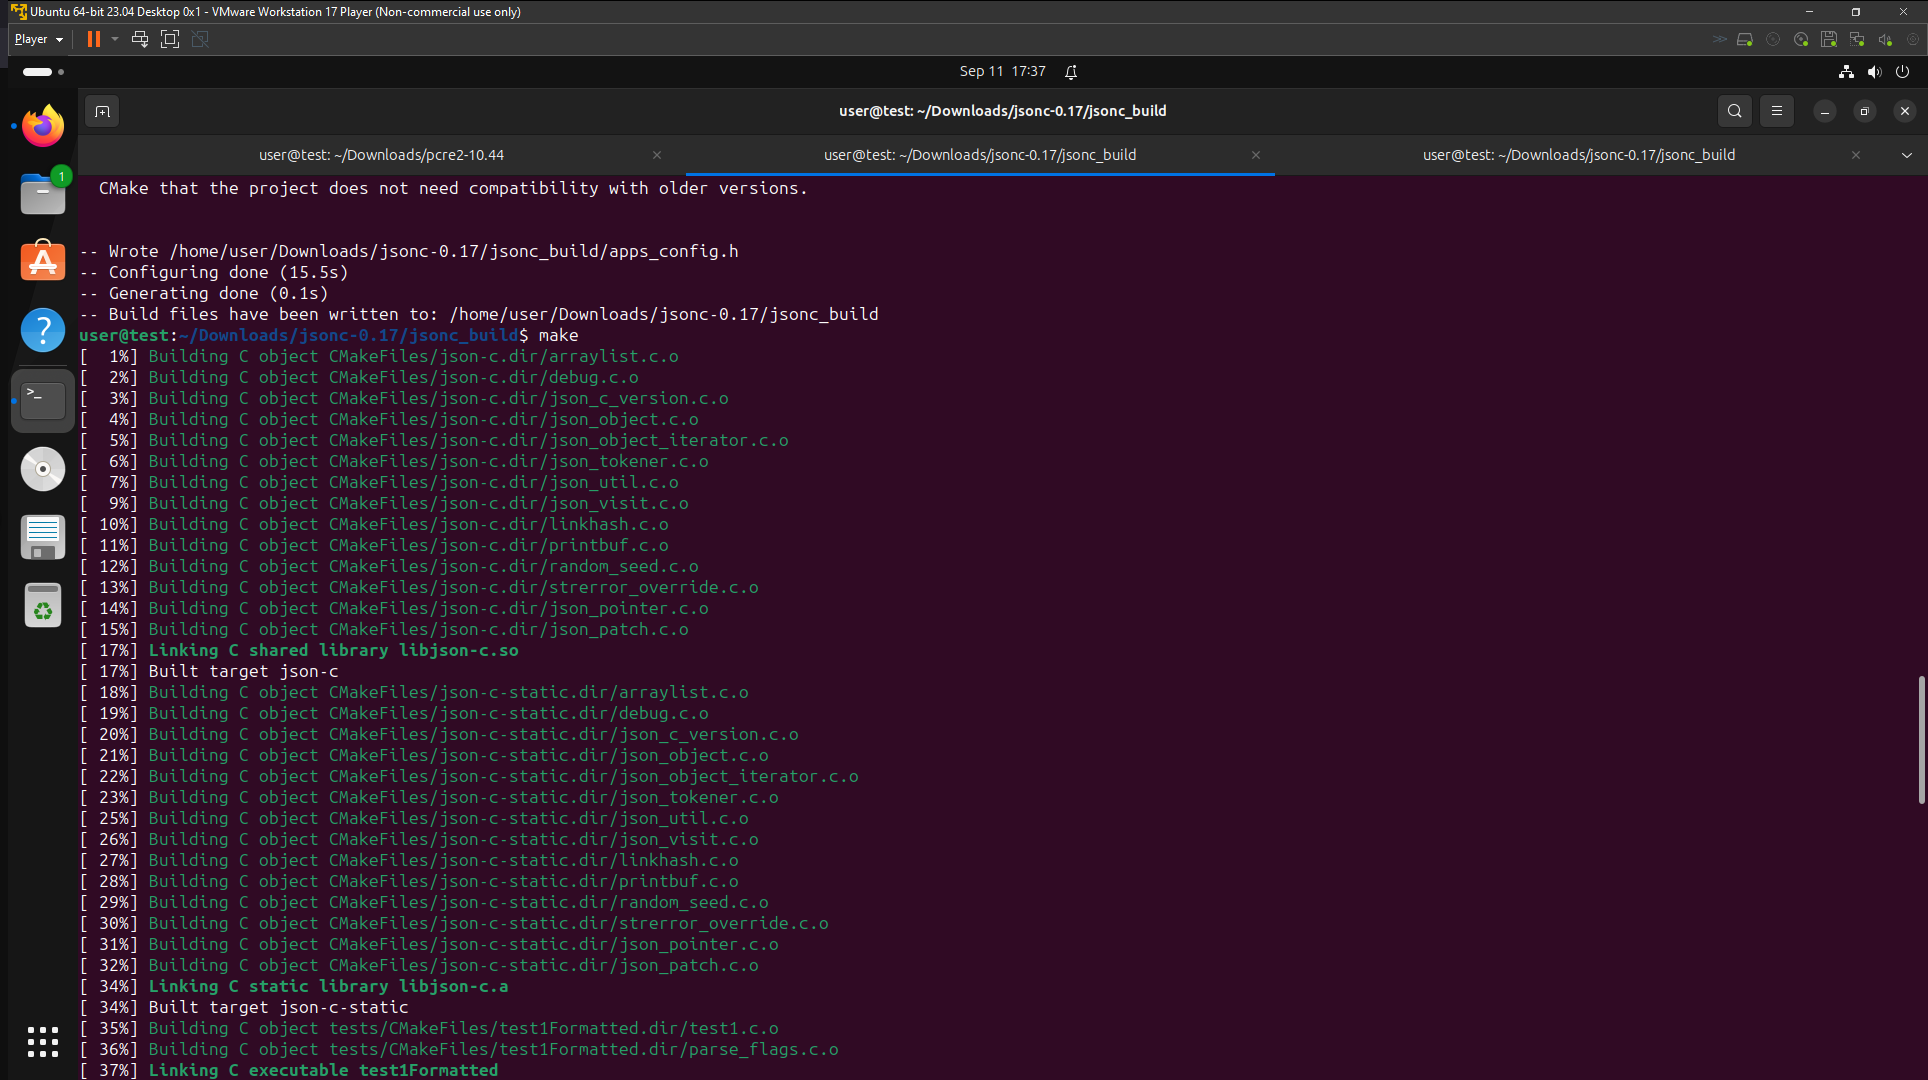
\includegraphics[width=0.9\textwidth]{../figure/jsonc_build_5.png}
    \end{figure}
\end{frame}

\begin{frame}
    \frametitle{Exercise: Build \texttt{json-c}}

    Finally, the build process is finished.

    \begin{figure}[H]
        \centering
        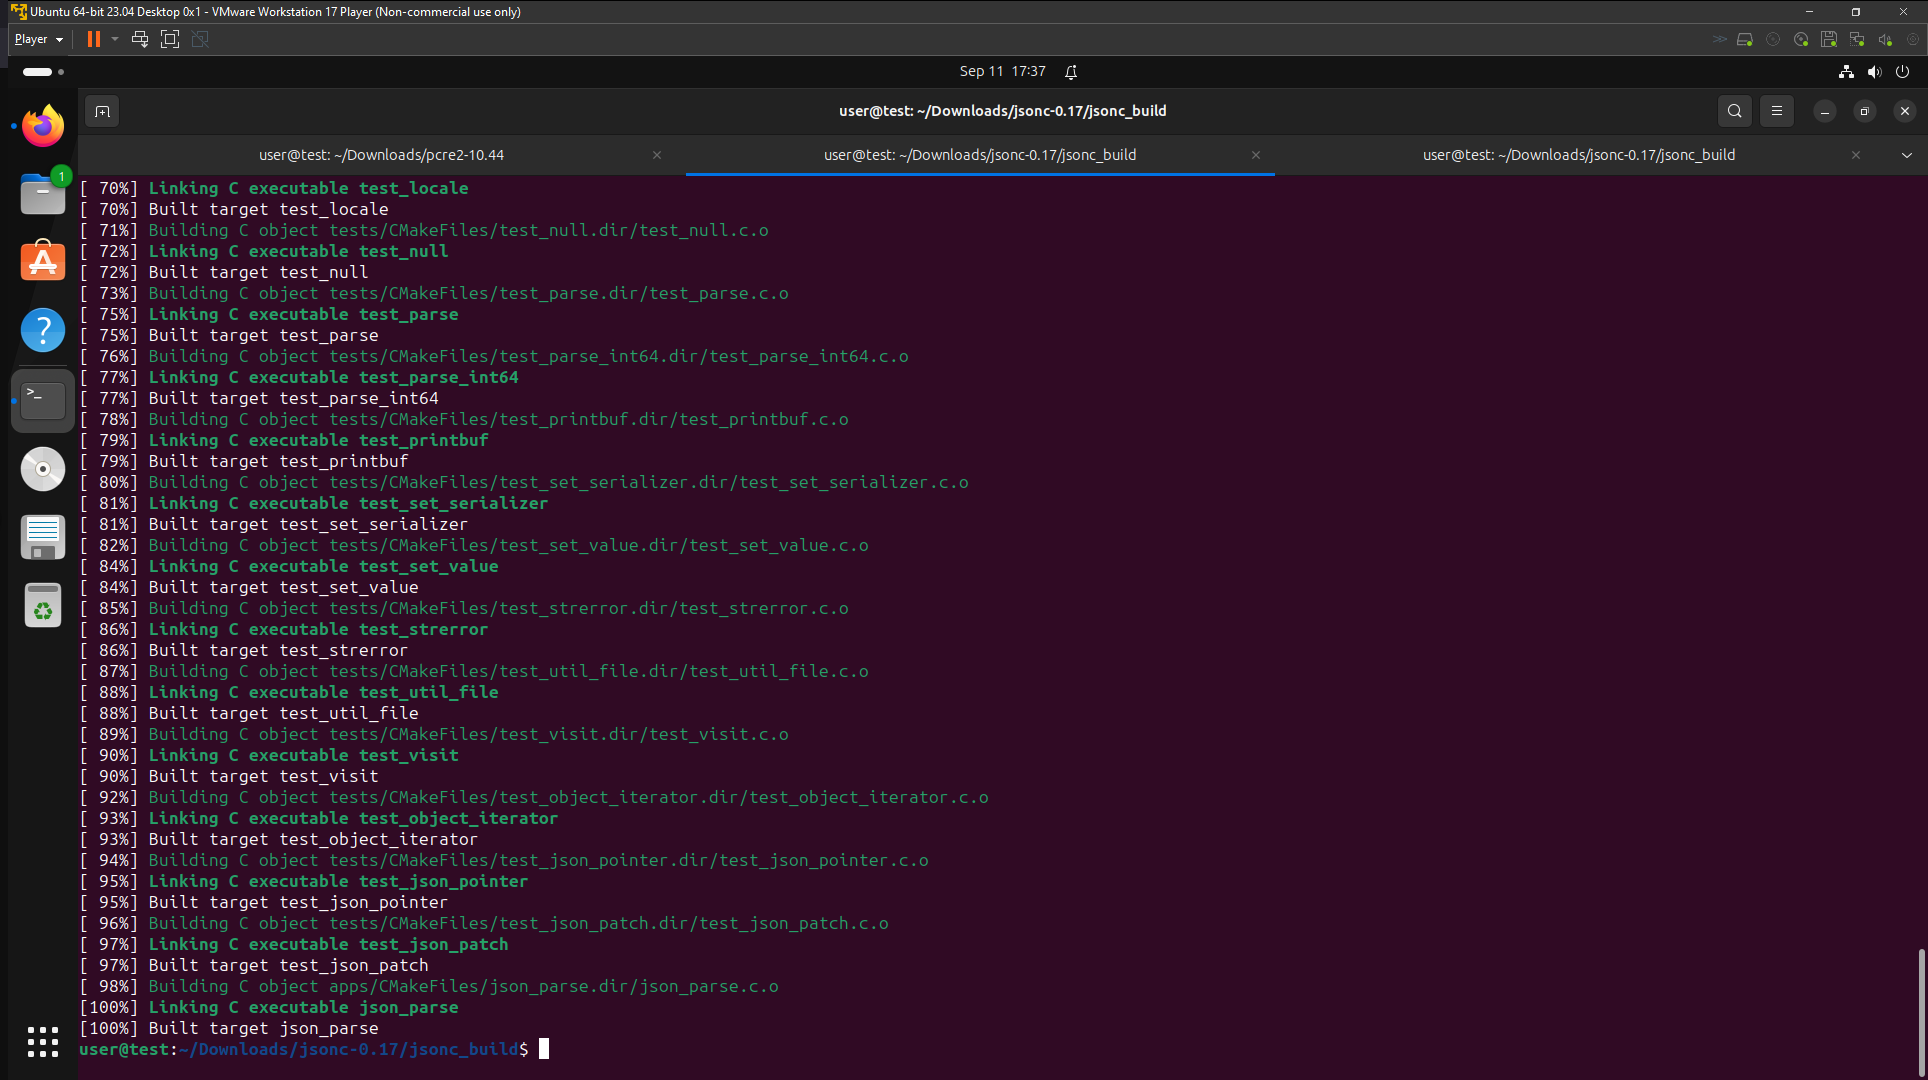
\includegraphics[width=0.9\textwidth]{../figure/jsonc_build_6.png}
    \end{figure}
\end{frame}

\begin{frame}
    \frametitle{Reference}

    \begin{itemize}
        \item \href{https://www.youtube.com/watch?v=YtiPCPtmZrs}{{[}Day 16{]} - Static and Dynamic Libraries (ar, objdump, ld, ldd) - Crash Course in C Programming by Mike Shah}
        \item \href{https://www.youtube.com/watch?v=Slfwk28vhws}{Write Better Code! | How to Create Shared Libraries in C/C++}
        \item \href{https://docs.redhat.com/en/documentation/red_hat_enterprise_linux/6/html/developer_guide/cmd-autotools-upstreamdocs\#cmd-autotools-upstreamdocs}{Red Hat Documentation 3.2.3. Autotools Documentation}
    \end{itemize}
\end{frame}


\end{document}
